\chapter*{Chương 6: Giải thích dựa trên mẫu dữ liệu}

Các phương pháp giải thích dựa trên mẫu dữ liệu lựa chọn các mẫu dữ liệu cụ thể trong tập dữ liệu để giải thích hành vi của các mô hình học máy hoặc để giải thích phân bố của dữ liệu.

Các phương pháp này chủ yếu có dạng nguyên mẫu (model-agnostic), bởi vì chúng có thể hoạt động trên bất cứ loại mô hình học máy nào. Sự khác nhau nhau so với các phương pháp model-agnostic có chăng là các phương pháp này giải thích một mô hình bằng cách chọn lựa các mẫu dữ liệu trong tập dữ liệu và không cần tạo tổng quan đặc trưng (feature summary) giống như phương pháp feature importance hay PDP. Các phương pháp giải thích dựa trên mẫu dữ liệu chỉ có ý nghĩa nếu ta có thể biểu diễn mẫu dữ liệu một cách mà con người có thể hiểu được. Với dữ liệu là ảnh, điều này không thành vấn đề, bởi vì ta có thể xem ảnh một cách trực tiếp. Nhìn chung, các phương pháp này sẽ làm việc tốt nếu các giá trị đặc trưng của mẫu dữ liệu chứa nhiều thông tin và có cấu trúc ví dụ như ảnh hoặc văn bản. Với dữ liệu dạng bảng (tabular), mọi thứ sẽ khó khăn hơn bởi vì một mẫu dữ liệu có thể chứa hàng trăm thậm chí hàng ngàn đặc trưng. Liệt kê tất các các giá trị đặc trưng để biểu diễn một mẫu dữ liệu trong trường hợp này sẽ không hiệu quả.

Các phương pháp giải thích dựa trên mẫu dữ liệu giúp con người hiểu về mô hình và tập dữ liệu đã được dùng cho việc huấn luyện. Chúng đặc biệt giúp ta nắm bắt các phân phối dữ liệu phức tạp. Nhưng giải thích dựa trên mẫu dữ liệu nghĩa là gì? Thực tình ta thường chúng các phương pháp này trong đời sống hàng ngày, hãy bắt đầu bằng vài ví dụ nhé.

Một bác sĩ trông thấy một bệnh nhân có triệu chứng ho và sốt nhẹ một cách không bình thường. Các triệu chứng này làm bác sĩ nhớ tới một bệnh nhân khác của cô ta vài năm về trước với các triệu chứng tương tự. Cô ấy nghi ngờ rằng bệnh nhân hiện tại có thể có cùng bệnh và cô ấy lấy mẫu máu của bệnh nhân để xét nghiệm.

Một nhà khoa học dữ liệu làm việc với một dự án mới cho một trong những khách hàng của anh ta: Phân tích các nhân tố nguy hiểm dẫn đến lỗi hoạt động của một máy sản xuất bàn phím. Nhà khoa học dữ liệu nhớ rằng một dự án tương tự anh ta đã làm và tái sử dụng một số phần của mã code từ dự án cũ đó bởi vì anh ta nghĩ rằng khách hàng muốn kiểu phân tích tương tự.

Một chú mèo con ngồi bên cửa sổ của một ngôi nhà hoang đang bị cháy. Lính cứu hỏa vừa tới nơi và một trong số họ suy nghĩ có nên lao vào đống lửa để cứu chú mèo hay không. Anh ta nhớ một số trường hợp tương tự  mà anh ta đã chứng kiến: các ngôi nhà gỗ cũ kĩ thường cháy âm ỉ và sẽ dễ dàng sập xuống bất cứ lúc nào. Bởi vậy, anh ta quyết định không lao vào, bởi vì nguy cơ là quá lớn. May mắn rằng, chú mèo đã nhảy ra khỏi cửa sổ và an toàn, cũng như không ai bị thương.

Những câu chuyện trên phản ánh cách con người chúng ta suy nghĩ trong các trường hợp thực tế. Đại thể của phương pháp giải thích dựa trên mẫu dữ liệu đó là: B giống với A và A dẫn đến Y, do đó tôi dự đoán rằng B cũng sẽ dẫn đến Y. Ta có thể thấy điều này với một số phương pháp học máy. Các cây quyết định phân tách dữ liệu thành các nốt dựa trên điểm tương đồng giữa các mẫu dữ liệu dựa vào các đặc trưng quan trọng cho việc dự đoán mục tiêu. Một cây quyết định tạo ra dự đoán cho một mẫu dữ liệu mới bằng cách tìm ra các mẫu dữ liệu tương đồng (tương đương với nốt cuối - terminal node) và trả về giá trị đầu ra trung bình của các mẫu dữ liệu đó như là các dự đoán. Với một mẫu dữ liệu mới, một mô hình k hàng xóm gần nhất (knn) định vị k hàng xóm gần nhất và trả về giá trị đầu ra trung bình của các hàng xóm như là dự đoán. Kết quả của một thuật toán k hàng xóm gần nhất có thể được giải thích bằng cách diễn giải k hàng xóm, và điều này, một lần nữa, chỉ có ý nghĩa nếu ta có thể biểu diễn chúng theo cách mà con người có thể hiểu được.

Chương này bao gồm các  phương pháp giải thích dựa trên mẫu dữ liệu:

- Giải thích phản chứng (counterfactual explanations): Cho ta biết mẫu dữ liệu cần thay đổi như thế nào để đầu ra cũng bị thay đổi. Bằng cách tạo ra các mẫu dữ liệu phản chứng, ta biết mô hình tạo ra dự đoán như thế nào và có thể giải thích cho các dự đoán riêng rẽ.

- Các mẫu dữ liệu đối kháng (adversarial examples): Là các phản chứng dùng để đánh lừa các mô hình học máy. Phần này tập trung vào việc thay đổi dự đoán và không đi kèm giải thích.

- Nguyên mẫu (prototypes): Là việc lựa chọn ra các mẫu dữ liệu đại diện từ một tập dữ liệu và ngoại lại (criticisms) là các mẫu dữ liệu không được bao hàm bởi các nguyên mẫu.

- Các mẫu dữ liệu có ảnh hưởng (influential instances): Là các mẫu dữ liệu quan trọng bậc nhất cho các tham số của một mô hình hoặc dự đoán. Việc xác định và phân tích các mẫu dữ liệu này giúp ta hiểu được các vấn đề trong tập dữ liệu, gỡ rối mô hình và nắm bắt hành vi của mô hình tốt hơn.

- Mô hình k hàng xóm gần nhất (k-nearest neighbors model): Là một dạng mô hình học máy khả diễn giải dựa trên các mẫu dữ liệu.

\section{Giải thích phản chứng - Counterfactual Explanations}
Một lời giải thích phản chứng mô tả một tình huống có dạng nhân quả dưới dạng: ``Nếu X không xảy ra, Y sẽ không xảy ra''. Ví dụ: ``Nếu tôi không uống một ngụm cà phê nóng này, tôi sẽ không bị bỏng lưỡi''. Sự kiện Y là tôi bị bỏng lưỡi; nguyên nhân X là tôi đã uống cà phê nóng. Suy nghĩ theo lối phản chứng đòi hỏi phải tưởng tượng ra một giả định mâu thuẫn với các sự kiện được quan sát (ví dụ, một thế giới trong đó tôi không uống cà phê nóng), do đó có tên là ``phản chứng''. Khả năng suy nghĩ ra những phản chứng khiến con người chúng ta thông minh hơn nhiều so với các loài động vật khác.

Trong học máy khả giải thích, những giải thích phản chứng có thể được sử dụng để giải thích các dự đoán của các trường hợp riêng lẻ. ``Sự kiện'' là kết quả dự đoán của một thể hiện  (instance), ``nguyên nhân'' là các giá trị đặc trưng cụ thể của thể hiện này được đưa vào mô hình và ``gây ra'' một dự đoán tất yếu. Được hiển thị dưới dạng biểu đồ, mối quan hệ giữa các yếu tố đầu vào và dự đoán rất đơn giản: Các giá trị đặc trưng gây ra sự dự đoán.

\begin{figure*}[h!]
	\centering
	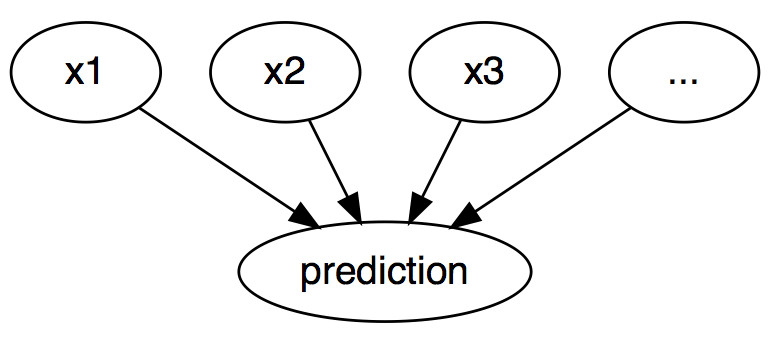
\includegraphics[scale=0.5]{images/graph.jpg}
    \label{fig:6.1}
    \caption{Mối quan hệ nhân quả giữa các yếu tố đầu vào của mô hình học máy và dự đoán, khi mô hình chỉ được xem như một hộp đen. Các đầu vào gây ra dự đoán (không nhất thiết phản ánh mối quan hệ nhân quả thực sự của dữ liệu).}
\end{figure*}

Ngay cả trong thực tế, mối quan hệ giữa các yếu tố đầu vào và kết quả được dự đoán có thể không phải là mối quan hệ nhân quả, chúng ta có thể xem đầu vào của một mô hình là nguyên nhân của dự đoán.

Với biểu đồ đơn giản này, thật dễ dàng để xem làm thế nào chúng ta có thể mô phỏng các phản chứng cho dự đoán của các mô hình học máy: Chúng ta chỉ cần thay đổi các giá trị đặc trưng của một thể hiện (instance) trước khi đưa ra dự đoán và chúng ta phân tích dự đoán thay đổi như thế nào. Chúng ta quan tâm đến các kịch bản trong đó dự đoán thay đổi theo cách có liên quan, như lật (flip) trong lớp dự đoán (ví dụ: đơn tín dụng được chấp nhận thành từ chối) hoặc trong đó dự đoán đạt đến ngưỡng nhất định (ví dụ: xác suất ung thư đạt 10\%). \textbf{Một giải thích phản chứng của dự đoán mô tả sự thay đổi nhỏ nhất trên các giá trị đặc trưng nhằm thay đổi dự đoán thành một giá trị được định trước.}

Có cả phương pháp giải thích phản chứng dạng mô hình mẫu (model-agnostic) và mô hình cụ thể (model-specific), nhưng trong chương này chúng ta chỉ tập trung vào các phương pháp mô hình mẫu - chỉ yêu cầu đầu vào và đầu ra (chứ không cần biết cấu trúc bên trong của các mô hình cụ thể). Các phương pháp này cũng sẽ tương tự chương mô hình mẫu, vì cách diễn giải có thể được biểu thị dưới dạng tóm tắt các sự khác biệt trong các giá trị đặc trưng (``thay đổi đặc trưng A và B để thay đổi dự đoán''). Nhưng một giải thích phản chứng tự nó là một mẫu dữ liệu mới, vì vậy nó nằm trong chương này (``bắt đầu từ thể hiện X, thay đổi A và B để có được một thể hiện phản chứng). Không giống như các nguyên mẫu (prototypes), các phản chứng không nhất thiết phải là các mẫu dữ liệu thực tế từ dữ liệu huấn luyện, mà có thể là một tổ hợp mới của các giá trị đặc trưng.

Trước khi thảo luận cách tạo nên các phản chứng, tôi muốn đề cập tới một số công dụng của phản chứng và một phản chứng được coi là tốt khi nào?

Trong ví dụ đầu tiên, Peter nộp đơn vay và bị từ chối bởi một phần mềm ngân hàng (chạy bởi học máy). Anh ấy tự hỏi tại sao đơn đăng ký của mình bị từ chối và làm thế nào để anh ấy có thể cải thiện cơ hội được vay. Câu hỏi ``tại sao'' có thể được hình thành như một phản chứng: Thay đổi nhỏ nhất đối với các đặc trưng (thu nhập, số thẻ tín dụng, độ tuổi, ...) sẽ thay đổi dự đoán từ bị từ chối thành được chấp thuận là gì? Một câu trả lời có thể là: Nếu Peter kiếm được thêm 10.000 Euro mỗi năm, thì anh ta sẽ được vay. Hoặc nếu Peter có ít thẻ tín dụng hơn và không bị vỡ nợ cách đây 5 năm, anh ta sẽ được vay. Peter sẽ không bao giờ biết lý do từ chối, vì ngân hàng không quan tâm đến sự minh bạch, nhưng đó là một câu chuyện khác.

Trong ví dụ thứ hai, ta muốn giải thích một mô hình dự đoán một đầu ra có giá trị liên tục với các giải thích phản chứng. Anna muốn cho thuê căn hộ của mình, nhưng cô không chắc phải đòi bao nhiêu cho căn hộ đó, vì vậy cô quyết định huấn luyện một mô hình học máy để dự đoán giá thuê. Tất nhiên, vì Anna là một nhà khoa học dữ liệu, đó là cách cô ấy giải quyết vấn đề của mình. Sau khi nhập tất cả các thông tin chi tiết về kích thước, vị trí, vật nuôi có được phép nuôi hay không, v.v., mô hình nói với cô ấy rằng cô ấy có thể tính phí 900 Euro. Cô ấy mong đợi từ 1000 Euro trở lên, nhưng cô ấy tin tưởng mô hình của mình và quyết định thay đổi các giá trị đặc trưng của căn hộ để xem cô ấy có thể cải thiện giá trị của căn hộ như thế nào. Cô phát hiện ra rằng căn hộ có thể được cho thuê với giá hơn 1000 Euro, nếu nó lớn hơn 15 m2. Rất thú vị nhưng không thể thực hiện được, bởi vì cô ấy không thể mở rộng căn hộ của mình. Cuối cùng, bằng cách chỉ điều chỉnh các giá trị tính năng trong tầm kiểm soát của cô ấy (bếp tích hợp có / không, vật nuôi được phép có / không, loại sàn, v.v.), cô ấy phát hiện ra rằng nếu cô ấy cho phép vật nuôi và cài đặt cửa sổ có cách nhiệt tốt hơn, cô ấy có thể tính phí 1000 Euro. Anna đã bằng cách nào đó làm việc với các phản chứng để thay đổi kết quả.

Phản chứng là những giải thích thân thiện với con người, bởi vì chúng trái ngược với thực tế hiện tại và vì chúng có tính chọn lọc, có nghĩa là chúng thường tập trung vào một số thay đổi nhỏ về tính năng. Nhưng phản chứng lại bị ``hiệu ứng Rashomon''. Rashomon là một bộ phim Nhật Bản kể về vụ giết hại một Samurai do những người khác nhau kể lại. Mỗi câu chuyện giải thích kết quả tốt như nhau, nhưng các câu chuyện mâu thuẫn với nhau. Điều tương tự cũng có thể xảy ra với các phản chứng, vì thường có nhiều cách giải thích phản chứng khác nhau. Mỗi phản chứng kể một ``câu chuyện'' khác nhau về cách đạt được một kết quả nhất định. Một phản chứng có thể nói thay đổi đặc điểm A, phản chứng khác có thể nói giữ nguyên A nhưng thay đổi đặc điểm B, đó là một mâu thuẫn. Vấn đề này có thể được giải quyết bằng cách trình bày tất cả các giải thích phản chứng hoặc dùng một tiêu chí để đánh giá các phản chứng và chọn giải thích tốt nhất.

Nói về tiêu chí, làm thế nào để chúng ta định nghĩa một giải thích phản chứng là tốt? Đầu tiên, người sử dụng giải thích phản chứng xác định sự thay đổi có liên quan trong dự đoán của một mẫu dữ liệu (thực tế ngược - alternative reality). Một yêu cầu đầu tiên rõ ràng là ta cần \textbf{một phản chứng tạo ra dự đoán càng gần với đầu ra định trước càng tốt}. Không phải lúc nào bạn cũng có thể tìm ra phản chứng với đầu ra cho trước. Ví dụ, trong bài toán phân loại có hai lớp, một lớp hiếm và một lớp phổ thông, mô hình có thể luôn phân loại một đầu vào là lớp phổ thông. Việc thay đổi các giá trị tính năng sao cho nhãn được dự đoán sẽ chuyển từ lớp phổ thông sang lớp hiếm có thể là điều không thể. Do đó, ta muốn nới lỏng yêu cầu rằng dự đoán phản chứng tế phải khớp chính xác với kết quả được xác định trước. Trong ví dụ phân loại, chúng ta có thể tìm ra một phản chứng trong đó xác suất dự đoán của loại hiếm được tăng lên 10\% thay vì 2\% hiện tại. Câu hỏi đặt ra là, những thay đổi tối thiểu nào trong các tính năng để xác suất dự đoán thay đổi từ 2\% thành 10\% (hoặc gần 10\%)? Một tiêu chí chất lượng khác là \textbf{phản chứng phải tương đồng nhất có thể với với mẫu dữ liệu gốc về mặt giá trị đặc trưng}. Khoảng cách giữa phản chứng và mẫu dữ liệu gốc có thể được đo, ví dụ, với khoảng cách Manhattan hoặc khoảng cách Gower nếu ta có cả các đặc trưng rời rạc và liên tục. Phản chứng không chỉ nên gần với mẫu dữ liệu gốc mà còn đòi hỏi \textbf{thay đổi càng ít đặc trưng càng tốt}. Để tính toán chất lượng của một giải thích phản chứng bằng một thông số cụ thể, ta có thể đơn giản đếm số lượng đặc trưng bị thay đổi, hoặc dùng giá trị khoảng $L_0$ (chuẩn) giữa phản chứng và mẫu dữ liệu gốc. Thứ ba, ta thường mong muốn tạo ra \textbf{nhiều giải thích phản chứng đa dạng} để chủ thể quyết định có thể tiếp cận với nhiều cách khả thi để tạo ra một kết quả định trước. Ví dụ, tiếp tục ví dụ về khoản vay của, một giải thích phảng chứng có thể đề xuất tăng gấp đôi thu nhập để được vay, trong khi một giải thích khác có thể gợi ý chuyển đến một thành phố lân cận và tăng thu nhập lên một khoản nhỏ để được vay. Có thể lưu ý rằng mặc dù phản chứng đầu tiên có thể thực hiện được đối với một số người, nhưng phản chứng thứ hai sẽ khả dĩ hơn rất nhiều. Do đó, bên cạnh việc cung cấp cho chủ thể quyết định những cách thức khác nhau để có được kết quả mong muốn, sự đa dạng còn cho phép các cá nhân ``đa dạng'' thay đổi các đặc trưng thuận tiện cho họ. Yêu cầu cuối cùng là \textbf{một phản chứng phải có các giá trị đặc trưng hợp lý}. Sẽ là phi lý nếu tạo ra một giải thích phản chứng cho ví dụ về giá thuê trong đó diện tích căn hộ là âm hoặc số phòng được đặt thành 200. Thậm chí còn tốt hơn nếu phản chứng có thể tuân theo phân phối chung của dữ liệu, ví dụ, một căn hộ có 10 phòng và 20 m2 không nên được coi là phản chứng (vì diện tích phòng quá nhỏ). Tốt nhất, nếu số mét vuông được tăng lên, thì việc tăng số lượng phòng cũng nên được đề xuất.

\subsection{Tạo ra giải thích phản chứng}
Một cách tiếp cận đơn giản nhất để tạo ra các giải thích phản chứng đó là tìm kiếm bằng cách thử và dò lỗi (trial and error). Cách tiếp cận này liên quan đến việc thay đổi ngẫu nhiên các giá trị đặc trưng của mẫu dữ liệu được quan tâm và dừng khi đạt được dự đoán đầu ra mong muốn. Như ví dụ khi Anna cố gắng thay đổi căn hộ của mình để có thể tính thêm tiền thuê. Tuy nhiên ta cũng có những cách tiếp cận tốt hơn. Đầu tiên, ta xác định một hàm mất mát dựa trên các tiêu chí đã đề cập ở trên. Hàm mất mát này lấy đầu vào là mẫu dữ liệu ta đang quan tâm, một phản chứng và đầu ra mong muốn. Sau đó, chúng ta có thể tìm ra giải thích phản chứng giúp giảm thiểu tổn thất này bằng cách sử dụng một thuật toán tối ưu. Nhiều phương pháp tiến hành theo cách này nhưng khác nhau về định nghĩa của hàm mất mát và phương pháp tối ưu hóa.

Sau đây, chúng ta tìm hiểu hai trong số chúng: thứ nhất, một của Wachter et al. (2017), người đã giới thiệu giải thích phản chứng như một phương pháp giải thích và thứ hai, phương pháp của Dandl et al. (2020) sử dụng cả bốn tiêu chí nêu trên.

\subsubsection{Phương pháp của Watcher et al. (2017)}
Wachter et al. đề xuất hàm mất mát sau:

$$L(x,x^\prime,y^\prime,\lambda)=\lambda\cdot(\hat{f}(x^\prime)-y^\prime)^2+d(x,x^\prime)$$

Thành phần đầu tiên là khoảng cách bậc hai giữa dự đoán của mô hình cho phản chứng $x^\prime$ và kết quả mong muốn $y^\prime$, mà người dùng phải xác định trước.Thành phần thứ hai là khoảng cách d giữa mẫu dữ liệu $x$ được giải thích và phản chứng $x^\prime$. Sự mất mát đo lường kết quả dự đoán của chứng khác bao xa so với kết quả được xác định trước và phản chứng khác bao xa so với mẫu dữ liệu quan tâm. Hàm khoảng cách d được định nghĩa là khoảng cách Manhattan có trọng số với độ lệch tuyệt đối trung vị nghịch đảo (Inverse mean absolute deviant - Inverse MAD) của mỗi đặc trưng.

$$d(x,x^\prime)=\sum_{j=1}^p\frac{|x_j-x^\prime_j|}{MAD_j}$$

Tổng khoảng cách là tổng của tất cả p khoảng cách theo đặc trưng, tức là sự khác biệt tuyệt đối của các giá trị đặc trưng giữa mẫu $x$ và mẫu $x^\prime$. Các khoảng cách theo đặc trưng được chia tỷ lệ bởi nghịch đảo của độ lệch tuyệt đối trung vị của đặc trưng $j$ trên toàn tập dữ liệu được xác định là:

$$MAD_j=\text{median}_{i\in{}\{1,\ldots,n\}}(|x_{i,j}-\text{median}_{l\in{}\{1,\ldots,n\}}(x_{l,j})|)$$

Trung vị của vectơ là giá trị mà tại đó một nửa giá trị vectơ lớn hơn và nửa còn lại nhỏ hơn. MAD tương đương với phương sai của một đặc trưng, nhưng thay vì sử dụng giá trị trung bình làm trung tâm và tính tổng trên các khoảng cách bình phương, ta sử dụng trung vị làm tâm và tổng trên các khoảng cách tuyệt đối. Hàm khoảng cách được đề xuất này có ưu điểm so với khoảng cách Euclide là nó mạnh hơn đối với các điểm ngoại lai. Việc chia tỷ lệ với MAD là cần thiết để đưa tất cả các đặc trưng về cùng một tỷ lệ - ví dụ cho dù bạn đo kích thước của một căn hộ theo mét vuông hay mét vuông, kết quả cũng không thay đổi.

Thông số $\lambda$ cân bằng khoảng cách của dự đoán (số hạng đầu tiên) với khoảng cách của các giá trị đặc trưng (số hạng thứ hai). Với mỗi $\lambda$, hàm mất mát trả về một phản chứng $x^\prime$ khác nhau. $\lambda$ càng lớn nghĩa là ta muốn phản chứng có dự đoán gần với kết quả mong muốn $y^\prime$, giá trị $\lambda$ càn thấp nghĩa là ta muốn $x^\prime$ giống với x về mặt các giá trị đặc trưng. Nếu $\lambda$ rất lớn, mẫu có dự đoán gần $y^\prime$ nhất sẽ được chọn, bất kể nó cách $x$ bao xa. Cuối cùng, người dùng phải quyết định cách cân bằng giữa yêu cầu rằng dự đoán cho chứng khớp với kết quả mong muốn với yêu cầu phản chứng giống với $x$. Các tác giả của phương pháp đề xuất thay vì chọn một giá trị cho $\lambda$ thì nên chọn một giá trị dung sai (tolerance) $\epsilon$ cho phép giới hạn khoảng cách từ dự đoán trên mẫu phản chứng tới $y^\prime$. Ràng buộc này có thể được biểu diễn như sau:

$$|\hat{f}(x^\prime)-y^\prime|\leq\epsilon$$

Để tối ưu hàm mất mát này, có thể sử dụng bất kỳ thuật toán tối ưu hóa phù hợp nào, chẳng hạn như Nelder-Mead. Nếu ta có thể tiếp cận gradient của mô hình học máy, ta có thể sử dụng các phương pháp tối ưu dựa trên gradient như ADAM. Mẫu $x$ được giải thích, đầu ra mong muốn $y^\prime$ và tham số dung sai $\epsilon$ phải được xác định trước. Hàm mất mát được tối ưu để tìm ra $x^\prime$ khi tăng giá trị $\lambda$ cho đến khi đầu ra nằm giá khoảng giá trị mong muốn (= trong tham số dung sai):

$$\arg\min_{x^\prime}\max_{\lambda}L(x,x^\prime,y^\prime,\lambda).$$

Nhìn chung, các bước để tạo ra phản chứng sẽ như sau:

1. Lựa chọn một mẫu $x$ để giải thích, đầu ra mong muốn $y^\prime$, và giá trị dung sai $\epsilon$ và một giá trị $\lambda$ đủ nhỏ.

2. Lấy một mẫu bất kỳ làm phản chứng khởi tạo.

3. Tối ưu hàm mất mát với phản chứng khởi tạo là điểm bắt đầu.

4. Khi $|\hat{f}(x^\prime)-y^\prime|>\epsilon$:

- Tăng $\lambda$.

- Tối ưu mất mát với phản chứng hiện tại là điểm bắt đầu.

- Trả về phản chứng tương ứng với giá trị mất mát nhỏ nhất.

5. Lặp lại các bước số 2 đến 4 và trả về danh sách các phản chứng mà tối ưu giá trị mất mát.

Phương pháp nêu trên có một số nhược điểm. Nó chỉ tính đến tiêu chí đầu tiên và tiêu chí thứ hai chứ không tính đến hai tiêu chí cuối cùng (``tạo ra các phản chứng chỉ với ít thay đổi về đặc trưng và các giá trị đặc trưng là hợp lệ''). Ta đương nhiên sẽ ưu tiên các phản chứng mà chỉ yêu cầu thay đổi một đặc trưng lên 10 đơn vị hơn là các phản chứng tăng 10 đặc trưng, mỗi đặc trưng một đơn vị. Các sự kết hợp phi thực tế của các đặc trưng cũng không bị trừng phạt trong hàm mất mát kiểu này.

Phương pháp này cũng không thể xử lý tốt với các dữ liệu có dạng hạng mục với nhiều cấp độ khác nhau. Các tác giả của phương pháp này đề xuất chạy phương pháp một cách riêng biệt cho từng tổ hợp các giá trị đặc trưng của các đặc trưng hạng mục, nhưng điều này sẽ dẫn đến sự bùng nổ về số lượng tổ hợp nếu ta có nhiều đặc trưng hạng mục với nhiều giá trị. Ví dụ: 6 đặc trưng hạng mục với 10 cấp độ có thể dẫn tới 1 triệu lượt chạy.

Bây giờ chúng ta hãy xem xét một cách tiếp cận khác để khắc phục những vấn đề này.

\subsubsection{Phương pháp của Dandl et al. (2020)}
Dandl et al. đề xuất tối ưu cùng lúc 4 hàm mất mát:

$$L(x,x',y',X^{obs})=\big(o_1(\hat{f}(x'),y'),o_2(x, x'),o_3(x,x'),o_4(x',X^{obs})\big)$$

Mỗi hàm mất mát từ $o_1$ tới $o_4$ tương ứng với một trong 4 tiêu chí nêu trên. Hàm mất mát đầu tiên $o_1$ phản ánh tiêu chí rằng dự đoán trên phản chứng $x^\prime$ nên gần giống với giá trị $y^\prime$ mong muốn. Do đó, ta cần tối ưu khoảng cách giữa $\hat{f}(x')$ và  $y^\prime$. Ở đây ta sử dụng công thức Manhattan (chuẩn $L_1$).

$$o_1(\hat{f}(x'),y')=\begin{cases}0&\text{if $\hat{f}(x')\in{}y'$}\\\inf\limits_{y'\in y'}|\hat{f}(x')-y'|&\text{else}\end{cases}$$

Hàm mục tiêu $o_2$ phản ánh rằng phản chứng của ta nên gần giống với mẫu dữ liệu $x$. Điều này được thể hiện bởi khoảng cách giữa $x^\prime$ và $x$ theo khoảng cách Gower:

$$o_2(x,x')=\frac{1}{p}\sum_{j=1}^{p}\delta_G(x_j, x'_j)$$

với p là số lượng đặc trưng. Giá trị $\delta_G$ phụ thuộc vào loại đặc trưng của $x_j$:

$$\delta_G(x_j,x'_j)=\begin{cases}\frac{1}{\widehat{R}_j}|x_j-x'_j|&\text{if $x_j$ numerical}\\\mathbb{I}_{x_j\neq{}x'_j}&\text{if $x_j$ categorical}\end{cases}$$

Ở đây đặc trưng dạng số là numerical và dạng hạng mục là categorical. Ta chia khoảng cách của một đặc trưng dạng số $j$ cho $\widehat{R}_j$, là dải giá trị, và thu được giá trị $\delta_G$ cho tất cả các đặc trưng giữa 0 và 1.

Khoảng cách Gower có thể dùng cho cả cả đặc trưng dạng số và hạng mục, nhưng không cân nhắc đến số lượng đặc trưng bị thay đổi. Do đó, ta tính số lượng đặc trưng bị thay đổi bằng hàm mục tiêu $o_3$ sử dụng chuẩn $L_0$.

$$o_3(x,x')=||x-x'||_0=\sum_{j=1}^{p}\mathbb{I}_{x'_j\neq x_j}.$$

Bằng cách tối ưu $o_3$, ta hướng tới tiêu chí thứ ba - số lượng đặc trưng bị thay đổi ít.

Hàm mục tiêu thứ tư $o_4$ phản ánh rằng phản chứng của ta nên có các giá trị đặc trưng hoặc các tổ hợp hợp lý. Ta có thể tính toán ``độ hợp lý'' của một mẫu dữ liệu bằng cách sử dụng tập huấn luyện hoặc một tập dữ liệu bất kỳ. Đặt tập dữ liệu này tên là $X^{obs}$. Như một phép xấp xỉ độ hợp lý (likelihood), $o_4$ tính toán khoảng cách Gower trung bình giữa $x^\prime$ và mẫu dữ liệu quan sát gần nhất $x^{[1]}\in{}X^{obs}$.

$$o_4(x',\textbf{X}^{obs})=\frac{1}{p}\sum_{j=1}^{p}\delta_G(x'_j,x^{[1]}_j)$$

So sánh với phương pháp của Wachter et al. thì $L(x,x',y',X^{obs})$ không có tham số cân bằng $\lambda$. Ta không muốn gộp cả bốn hàm mục tiêu này thành một bằng cách cộng tổng và nhân trọng số chúng, điều ta muốn là tối ưu tất cả bốn hàm mục tiêu này cùng một lúc.

Làm thế nào chúng ta có thể làm được điều đó? Ta sử dụng thuật toán di truyền sắp xếp không thống trị (Nondominated Sorting Genetic Algorithm) hoặc ngắn gọn hơn là NSGA-II. NSGA-II là một thuật toán lấy cảm hứng từ việc áp dụng định luật của Darwin về chọn lọc tự nhiên (survival of the fittest). Ta biểu diễn  mức độ ``mạnh'' của một phản chứng bằng một vectơ chứa giá trị của các hàm mục tiêu $(o_1,o_2,o_3,o_4)$. Phản chứng càng có giá trị vector thấp thì nó càng \textbf{mạnh}.

Thuật toán bao gồm bốn bước lặp đi lặp lại cho tới khi các với điều kiện nhất định (ví dụ số lượng vòng lặp/tạo). Hình sau đây trực quan hóa 4 bước cho việc tạo ra phản chứng. 

\begin{figure*}[h!]
	\centering
	\includegraphics[scale=0.3]{images/cfexp-nsgaII.jpg}
	\label{fig:6_2}
	\caption{Các bước tạo ra phản chứng sử dụng thuật toán NSGA-II.}
\end{figure*}

Trong lần tạo phản chứng thứ nhất, một nhóm các ứng viên cho phản chứng được khởi tạo bằng cách thay đổi ngẫu nhiên một số đặc trưng so với mẫu $x$ đang được giải thích. Theo ví dụ về tín dụng ở trên, một phản chứng có thể đề xuất tăng thu nhập thêm 30.000 Euro trong khi một đối tượng khác đề xuất không có vỡ nợ trong 5 năm qua và giảm 10 tuổi. Tất cả các giá trị đặc trưng khác đều bằng giá trị của $x$. Mỗi ứng viên sau đó được đánh giá bằng cách sử dụng bốn hàm mục tiêu ở trên. Trong số đó, ta chọn ngẫu nhiên một số ứng viên, trong đó các ứng viên có độ mạnh lớn hơn có nhiều khả năng được chọn hơn. Các ứng cử viên được kết hợp lại theo cặp để tạo ra những phản chứng con giống với chúng bằng cách lấy trung bình các giá trị đặc trưng số của chúng hoặc bằng cách loại bỏ các đặc trưng dạng hạng mục. Ngoài ra, ta thay đổi một chút các giá trị đặc trưng của phản chứng con để khám phá toàn bộ không gian đặc trưng.

Từ hai nhóm được sinh ra, gồm một phản chứng cha và một phản chứng con, ta chỉ muốn một nửa tốt nhất bằng cách sử dụng hai thuật toán sắp xếp. Thuật toán sắp xếp NSGA sắp xếp các ứng viên theo các giá trị của hàm mục tiêu $(o_1,o_2,o_3,o_4)$ (objective values) của chúng. Nếu các ứng viên mạnh như nhau, thuật toán phân bố đều mật độ ước lượng (crowding distance sorting algorithm) sẽ sắp xếp các ứng viên theo mức độ đa dạng của chúng.

Với kết quả của hai thuật toán sắp xếp, ta chọn một nửa lượng ứng cử viên có triển vọng nhất và/hoặc đa dạng nhất. Ta lại sử dụng tập ứng viên này cho lần tạo phản chứng tiếp theo và bắt đầu lại với quá trình chọn lọc, tái tổ hợp và biến đổi. Bằng cách lặp đi lặp lại các bước, ta hy vọng sẽ có được một tập hợp đa dạng các ứng viên triển vọng với giá trị của hàm mục tiêu thấp. Từ bộ này, ta có thể chọn những phản chứng mà ta hài lòng nhất hoặc có thể đưa ra một bản tóm tắt về tất cả các phản chứng bằng cách đánh dấu những tính năng nào và tần suất đã được thay đổi.

\subsection{Ví dụ}

Ví dụ dưới đây dựa trên ví dụ về điểm tín dụng trong Dandl et al. (2020). Tập dữ liệu German Credit có thể được tìm thấy tại trang Kaggle. Các tác giả đã huấn luyện một mô hình SVM với nhân bán kính cơ sở (radial basis kernel) để dự đoán độ rủi ro tín dụng của một khách hàng. Tập dữ liệu này có 522 mẫu hoàn chỉnh và 9 đặc trưng chứa thông tin tín dụng và khách hàng. Mục tiêu là tìm ra các giải thích phản chứng (counterfactual) cho một khách hàng với các giá trị đặc trưng trong bảng \ref{tab:german-credit}.

\begin{table}[]
\caption{}
\centering
\label{tab:german-credit}
\begin{tabular}{|c|c|c|c|c|c|c|c|c|}
\hline
age & sex & job       & housing & savings & checking & amount & duration & purpose \\ \hline
58  & f   & unskilled & free    & little  & little   & 6143   & 48       & car     \\ \hline
\end{tabular}
\end{table}

Mô hình SVM dự đoán rằng phụ nữ có rủi ro tín dụng thấp với xác suất 24,2\%. Các phản chứng nên trả lời câu hỏi: Các đặc trưng đầu vào cần phải thay đổi như thế nào để có xác suất dự đoán lớn hơn 50\%? Bảng \ref{tab:german-credit2} chứa 10 phản chứng tốt nhất:

\begin{table}[]
\caption{}
\centering
\label{tab:german-credit2}
\begin{tabular}{|l|l|l|l|l|l|l|l|l|}
\hline
\multicolumn{1}{|c|}{\textbf{age}} & \multicolumn{1}{c|}{\textbf{sex}} & \multicolumn{1}{c|}{\textbf{job}} & \multicolumn{1}{c|}{\textbf{amount}} & \multicolumn{1}{c|}{\textbf{duration}} & \multicolumn{1}{c|}{\textbf{$o_2$}} & \multicolumn{1}{c|}{\textbf{$o_3$}} & \multicolumn{1}{c|}{\textbf{$o_4$}} & \multicolumn{1}{c|}{\textbf{$\hat{f}(x')$}} \\ \hline
                                   &                                   & skilled                           &                                      & -20                                    & 0.108                          & 2                              & 0.036                          & 0.501                          \\ \hline
                                   &                                   & skilled                           &                                      & -24                                    & 0.114                          & 2                              & 0.029                          & 0.525                          \\ \hline
                                   &                                   & skilled                           &                                      & -22                                    & 0.111                          & 2                              & 0.033                          & 0.513                          \\ \hline
-6                                 &                                   & skilled                           &                                      & -24                                    & 0.126                          & 3                              & 0.018                          & 0.505                          \\ \hline
-3                                 &                                   & skilled                           &                                      & -24                                    & 0.120                          & 3                              & 0.024                          & 0.515                          \\ \hline
-1                                 &                                   & skilled                           &                                      & -24                                    & 0.116                          & 3                              & 0.027                          & 0.522                          \\ \hline
-3                                 & m                                 &                                   &                                      & -24                                    & 0.195                          & 3                              & 0.012                          & 0.501                          \\ \hline
-6                                 & m                                 &                                   &                                      & -25                                    & 0.202                          & 3                              & 0.011                          & 0.501                          \\ \hline
-30                                & m                                 & skilled                           &                                      & -24                                    & 0.285                          & 4                              & 0.005                          & 0.590                          \\ \hline
-4                                 & m                                 &                                   & -1254                                & -24                                    & 0.204                          & 4                              & 0.002                          & 0.506                          \\ \hline
\end{tabular}
\end{table}

Năm cột đầu tiên chứa các đề xuất thay đổi đặc trưng (chỉ các đặc trưng đã thay đổi được hiển thị), ba cột tiếp theo hiển thị các giá trị của hàm mục tiêu (objective values) ($o_1$ bằng 0 trong mọi trường hợp) và cột cuối cùng hiển thị xác suất dự đoán.

Tất cả các phản chứng đều có xác suất dự đoán lớn hơn 50\% và không chi phối lẫn nhau. Sự không chi phối (non-dominated) có nghĩa là không có phản chứng nào mà giá trị của cả 4 hàm mục tiêu đều nhỏ hơn 4 giá trị tương ứng của một phản chứng khác. Chúng ta có thể coi các phản chứng như một tập hợp các giải pháp mang tính đánh đổi (trade-off solutions).

Tất cả đều đề xuất giảm thời hạn từ 48 tháng xuống tối thiểu 23 tháng, một số đề xuất rằng người vay nên có tay nghề cao. Một số phản chứng còn đề nghị thay đổi giới tính từ nữ sang nam, cho thấy mô hình thiên vị giới tính. Sự thay đổi này luôn đi kèm với việc giảm tuổi trong khoảng từ 1 đến 30 tuổi. Chúng ta có thể thấy mặc dù một số phản chứng đề xuất thay đổi đối với cả 4 đặc trưng, nhưng các phản chứng này rất gần với mẫu ta đang xét trong bảng \ref{tab:german-credit}.

\subsection{Ưu điểm}
\textbf{Việc giải thích bằng phản chứng rất rõ ràng}. Nếu các giá trị đặc trưng của một đối tượng được thay đổi theo phản chứng, thì dự đoán sẽ thay đổi thành dự đoán đã xác định trước (predefined prediction). Do không có thêm giả định, mô hình không có rủi ro như các phương pháp như LIME, trong đó chúng ta không rõ chúng ta nên ngoại suy mô hình cục bộ bao xa để tạo tính khả giải thích.

Phương pháp phản chứng tạo ra một mẫu dữ liệu (instance) mới, nhưng ta cũng có thể tổng quan hóa một phản chứng thông qua các đặc trưng đã bị thay đổi. Điều này cung cấp \textbf{hai lựa chọn cho việc diễn giải kết quả}. Ta có thể diễn giải mẫu dữ liệu phản chứng hoặc đánh dấu các đặc trưng nào đã được thay đổi giữa mẫu dữ liệu quan tâm và mẫu dữ liệu phản chứng.

\textbf{Phương pháp phản chứng không yêu cầu quyền truy cập vào dữ liệu hoặc mô hình}. Nó chỉ yêu cầu truy nhập vào hàm dự đoán của mô hình. Ví dụ, hàm dự đoán hoạt động thông qua API web. Điều này có ích cho các công ty được kiểm toán bởi bên thứ ba hoặc giải thích cho người dùng mà không tiết lộ mô hình hoặc dữ liệu. Công ty quan tâm đến việc bảo vệ mô hình và dữ liệu vì bí mật thương mại hoặc lý do bảo vệ dữ liệu. Giải thích phản chứng đưa ra sự cân bằng giữa giải thích các dự đoán của mô hình và bảo vệ lợi ích của chủ sỡ hữu mô hình.

\textbf{Phương pháp này cũng hoạt động với các hệ thống không sử dụng học máy}. Chúng ta có thể tạo phản chứng cho bất kỳ hệ thống nào nhận đầu vào và trả đầu ra. Hệ thống dự đoán giá thuê căn hộ cũng bao gồm các đặc trưng thủ công và các giải thích phản chứng vẫn hoạt động được tốt.

\textbf{Phương pháp giải thích phản chứng tương đối dễ thực hiện}. Vì nó về cơ bản là một hàm mất mát (loss function) (với một hoặc nhiều mục tiêu) có thể được tối ưu hóa với các gói tối ưu hóa tiêu chuẩn. Một số chi tiết có thể bổ sung như giới hạn giá trị đặc trưng trong khoảng có ý nghĩa (ví dụ: kích thước căn hộ trong khoảng số dương).

\subsection{Nhược điểm}
\textbf{Đối với mỗi trường hợp, bạn thường sẽ tìm thấy nhiều lời giải thích phản chứng (hiệu ứng Rashomon)}. Hầu hết mọi người cần lời giải thích đơn giản hơn là phức tạp trong thế giới thực. Đó cũng là một thách thức. Giả sử ta đã tạo ra 23 giải thích phản chứng cho một mẫu dữ liệu. Liệu chúng ta đã báo cáo tất cả? Liệu ta đã báo cáo kết quả tốt nhất? Điều gì sẽ xảy ra nếu tất cả đều tương đối ``tốt'', nhưng rất khác nhau? Những câu hỏi này phải được trả lời riêng cho mỗi tình huống. Việc có nhiều giải thích phản chứng có thể có lợi, bởi vì sau đó ta có thể chọn lại những giải thích tương ứng với tình huống trước đây.

\subsection{Phần mềm và các phương pháp khác}
Phương pháp giải thích phản chứng đa mục tiêu (multi-objective counterfactual explanation) của Dandl et al. được triển khai trên Github.

Trong gói Python, các tác giả từ Alibi đã triển khai một phương pháp phản chứng đơn giản với một phương pháp mở rộng sử dụng các lớp nguyên mẫu để cải thiện tính khả diễn giải và hội tụ của đầu ra thuật toán.

Karimi et al. (2019) triển khai thuật toán MACE trên Github. Họ đã dịch các tiêu chí cần thiết cho các phản chứng thích hợp thành các công thức logic và sử dụng các bộ giải thỏa mãn (satisfiability solvers) để tìm ra các phản chứng thỏa mãn.

Mothilal et al. (2020) đã phát triển DiCE (Giải thích phản chứng đa dạng) (Diverse Counterfactual Explanation) để tạo ra một tập hợp đa dạng các giải thích phản chứng dựa trên các quá trình điểm định thức (determinantal point processes). Hiện tại, DiCE chỉ hoạt động cho các mô hình có thể đạo hàm (differentiable models) được vì nó sử dụng gradient descent để tối ưu hóa.

Một cách khác để tìm kiếm phản chứng là thuật toán Hình cầu phát triển (Growing Spheres) của Laugel et. al (2017). Họ không sử dụng từ phản chứng trong bài báo của họ, nhưng phương pháp khá giống nhau. Họ cũng xác định một hàm mất mát ưu tiên các phản chứng với càng ít thay đổi trong các giá trị đặc trưng càng tốt. Thay vì trực tiếp tối ưu hóa hàm số, trước tiên họ đề xuất vẽ một hình cầu xung quanh điểm quan tâm, lấy mẫu các điểm trong hình cầu đó và kiểm tra xem một trong các điểm lấy mẫu có mang lại dự đoán mong muốn hay không. Sau đó, ta thu nhỏ hoặc mở rộng hình cầu tương ứng cho đến khi tìm thấy một phản chứng.

Neo (Anchors) của Ribeiro et. al (2018) đi ngược lại với các phản chứng, xem chương về các quy tắc phạm vi (Scoped Rules).

\clearpage

\section{Các mẫu dữ liệu đối kháng - Adversarial examples} 

Một mẫu dữ liệu đối kháng là một mẫu có các thay đổi nhỏ trong giá trị đặc trưng có chủ đích nhằm đánh lừa mô hình học máy. Khuyến khích bạn đọc trước chương Giải thích phản chứng (chương 6.1), vì hai loại dữ liệu này khá tương đồng. Các mẫu dữ liệu đối kháng chính là các mẫu dữ liệu phản chứng với mục đích đánh lừa mô hình mà không phải để giải thích.

Tại sao chúng ta cần quan tâm đến các mẫu dữ liệu đối kháng? Các mẫu dữ liệu đối kháng làm cho mô hình học máy ``dễ bị tổn thương'' (vulnerable), như trong các kịch bản sau đây.

- Một xe hơi tự lái tông vào một chiếc xe khác vì nó bỏ qua một biển báo dừng (stop sign). Một ai đó đã đặt một hình khác lên trên cái biển báo, lúc này biển báo vẫn có thể nhận diện bởi mắt người chỉ có điều có thêm một chút đất bẩn. Trên thực tế, nó được thiết kế cho phần mềm nhận diện biển báo của xe hơi tự hành.

- Một bộ phát hiện thư rác không thể phân loại thư giác. Các thư rác này được thiết kế giống như một email bình thường, nhưng với ý đồ lừa đảo người nhận.

- Một máy quét chạy bằng học máy quét các vali để tìm vũ khí tại sân bay. Một con dao đã được tạo nên trông giống một chiếc ô để tránh sự nhận diện của hệ thống.

Chúng ta hãy xem xét một số cách để tạo ra các mẫu dữ liệu đối kháng.

\subsection{Các phương pháp và ví dụ}

Có nhiều phương pháp để tạo ra các mẫu dữ liệu đối kháng. Hầu hết các cách tiếp cận đề xuất việc tối thiểu hóa khoảng cách giữa mẫu dữ liệu đối kháng và mẫu gốc, trong khi thay đổi dự đoán thành các kết quả mong muốn (đối kháng). Một số phương pháp yêu cầu can thiệp đến gradient của mô hình, và tất nhiên chỉ hoạt động trên các mô hình dựa trên gradient như các mạng nơ-ron. Những phương pháp khác chỉ yêu cầu can thiệp đến hàm dự đoán, hoạt động trên các phương pháp mô hình mẫu (model-agnostic). Các phương pháp trong phần này tập trung vào bài toán phân loại hình ảnh với mạng nơ-ron sâu. Các mẫu dữ liệu đối kháng cho hình ảnh là các hình ảnh với pixel nhiễu có chủ ý với mục đích đánh lừa mô hình. Các mẫu dữ liệu đối kháng chứng minh rằng các mạng nơ-ron sâu có thể bị đánh lừa dễ dàng như thế nào bởi các hình ảnh mà tưởng chừng như bình thường với con người. Nếu bạn chưa bao giờ nhìn thấy các mẫu dữ liệu như vậy, bạn có thể bị bất ngờ, bởi vì sự thay đổi trong các dự đoán là khó có thể nhận biết đối với quan sát của con người. Các mẫu dữ liệu đối kháng giống như là ảo ảnh quang học với máy móc.

\paragraph{Có thứ gì đó không đúng với chú chó của tôi}
Szegedy et al. (2013) đã sử dụng phương pháp tối ưu dựa trên gradient trong bài báo ``Intriguing properties of neural networks'' để tìm các mẫu dữ liệu đối kháng cho các mạng học sâu trong hình \ref{fig:6_3}

\begin{figure*}[h!]
	\centering
	\includegraphics[scale=0.5]{images/adversarial-examples.jpg}
	\label{fig:6_3}
	\caption{Các mẫu dữ liệu đối kháng đối với với mạng AlexNet bởi Szegedy et al. (2013). Tất cả hình trên cột trái là đã được phân loại chính xác. Cột giữa hiển thị nhiễu được thêm vào hình ảnh để tạo thành các hình trong cột phải, tất cả được phân loại (không chính xác) là “Đà điểu”. ``Intriguing properties of neural networks''.}
\end{figure*}

Các mẫu dữ liệu đối kháng này được sinh ra bởi tối thiểu hóa hàm nhiễu sau với $r$:

\[loss(\hat{f}(x+r),l)+c\cdot|r|\]

Trong công thức này, $x$ là hình ảnh (đại diện bởi một vector của các pixel), $r$ là sự thay đổi đối với các pixel đó để tạo ra một hình ảnh đối kháng ($x+r$ tạo ra một hình mới), $l$ là dự đoán mong muốn, và tham số $c$ được sử dụng để làm cân bằng khoảng cách giữa các hình ảnh và khoảng cách giữa các dự đoán. Biểu thức thứ nhất là khoảng cách giữa dự đoán đầu ra trên mẫu dữ liệu đối kháng với lớp $l$ mong muốn, biểu thức thứ hai đo khoảng cách giữa mẫu dữ liệu đối kháng với ảnh gốc. Công thức trên hầu như giống với hàm mất mát để tạo ra các giải thích phản chứng. Có thêm một số ràng buộc cho $r$ để các giá trị pixel nằm giữa 0 và 1. Tác giả đề xuất để giải quyết bài toán tối ưu này bằng phương pháp L-BFGS, một thuật toán tối ưu hoạt động với các gradient.

\paragraph{Xáo trộn gấu trúc: Fast gradient sign method)}

Goodfellow et al. (2014) đã phát minh ra phương pháp FGSM cho việc sinh ra các hình ảnh đối kháng. Phương pháp này sử dụng gradient của mô hình gốc để tìm mẫu dữ liệu đối kháng. Hình ảnh gốc $x$ được thay đổi bởi việc thêm hoặc bớt đi một nhiễu nhỏ $e$ cho mỗi pixel. Việc ta thêm hoặc bớt $e$ phụ thuộc vào dấu của gradient cho các pixel là dương hoặc âm. Thêm các nhiễu theo hướng của gradient nhằm mục đích làm cho mô hình phân loại sai hình ảnh đó.

Công thức dưới đây mô tả FGSM:

\[x^\prime=x+\epsilon\cdot{}sign(\bigtriangledown_x{}J(\theta,x,y))\]

Trong đó $\bigtriangledown_x{}J$ là gradient của hàm mất mát của mô hình tương ứng với vector pixel đầu vào $x$, $y$ là vector nhãn đúng cho $x$ và $\theta$ là vector trọng số mô hình. Từ vector gradient (cùng có kích thước giống như vector của các pixel đầu vào) ta chỉ cần dấu: Dấu của gradient là dương (+1) nếu sự tăng cường độ pixel làm tăng giá trị hàm mất mát (độ lệch mà mô hình tạo ra) và âm (-1) nếu sự giảm đi của cường độ pixel làm giảm hàm mất mát. Mô hình dễ bị tấn công khi một mạng nơ-ron coi mối quan hệ giữa cường độ pixel đầu vào và đầu ra là tuyến tính. Đặc biệt, các kiến trúc mạng nơ-ron thiên về tuyến tính, như là LSTMs, mạng Maxout, mạng với hàm kích hoạt là ReLU hay các thuật toán học máy tuyến tính khác như hồi quy tuyến tính là dễ bị tấn công bởi phương pháp FGSM. Sự tấn công được thực hiện bởi phép ngoại suy. Liên kết tuyến tính giữa cường độ pixel đầu vào và đầu ra là nguyên nhân của việc các mô hình dễ bị tấn công bởi các ngoại lai (outlier), mẫu dữ liệu mà có thể được tạo ra bằng cách dịch chuyển giá trị pixel vào khu vực ngoài vùng phân phối dữ liệu hiện tại. Tôi mong rằng các mẫu dữ liệu đối kháng là chuyên biệt cho các kiến trúc mạng nơ-ron, nghĩa là chỉ một vài kiến trúc mạng bị đánh lừa bởi chúng. Nhưng hóa ra, ta có thể tái sử dụng các mẫu dữ liệu đối kháng để đánh lừa mạng với một kiến khác được huấn luyện trên cùng một nhiệm vụ (ví dụ phân loại hình ảnh).

Goodfellow et al. (2014) đã đề xuất việc thêm các mẫu dữ liệu đối kháng vào dữ liệu huấn luyện để tăng sức mạnh của mô hình.

\paragraph{Một con sứa... Không, chờ đã. Là một bồn tắm: Tấn công trên 1 pixel}

Phương pháp được phát minh bởi Goodfellow et al. (2014) yêu cầu nhiều pixel thay đổi cùng lúc một lượng nhỏ. Nhưng chuyện gì xảy ra nếu ta chỉ có thể thay đổi một pixel duy nhất? Ta có khả năng đánh lừa mô hình học máy không? Su et al. (2019) đã chỉ ra rằng thực chất có thể đánh lừa việc phân loại hình ảnh bằng cách thay đổi duy nhất một pixel.

\begin{figure*}[h!]
	\centering
	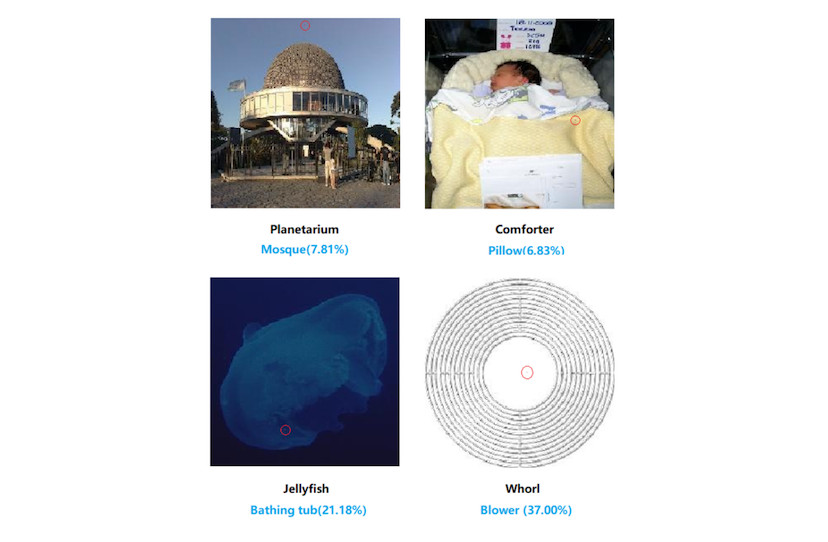
\includegraphics[scale=0.3]{images/adversarial-1pixel.png}
	\label{fig:6_4}
	\caption{Bằng việc thay đổi chủ ý một pixel, một mạng nơ-ron đã huấn luyện trên ImageNet có thể bị đánh lừa để dự đoán sai lớp thay vì lớp đúng ban đầu.}
\end{figure*}

Tương tự như các phản chứng, tấn công trên 1-pixel tìm một mẫu dữ liệu $x^\prime$ mà nó gần với hình ảnh gốc $x$, nhưng thay dự đoán tới một đầu ra đối kháng. Tuy nhiên, định nghĩa của việc ``gần'' là khác: chỉ một pixel có thể thay đổi. Tấn công trên 1-pixel sử dụng phép vi phân để tìm ra pixel nào được thay đổi và cách thay đổi. Phép vi phân này được lấy cảm hứng từ tiến hóa sinh học của các loài. Một nhóm các ứng viên cho pixel được sửa đổi được tái tổ hợp liên tục cho đến khi đáp án được tìm ra. Mỗi ứng viên ứng với một pixel bị thay đổi và nó được thể hiện bởi một vector với 5 thành phần: giá trị trục x, y và màu đỏ, xanh lá cây và xanh da trời (RGB). Việc tìm kiếm bắt đầu với 400 ứng cử viên và tạo ra một thế hệ các giải pháp ứng cử viên (con) mới từ thế hệ cha sử dụng công thức sau đây:

$$x_{i}(g+1)=x_{r1}(g)+F\cdot(x_{r2}(g)-x_{r3}(g))$$

Trong đó $x_i$ là một thành phần của một ứng viên (có thể là toạ độ x, tọa độ y, đỏ, xanh lá cây và xanh da trời), $g$ là thế hệ hiện tại, $F$ là tham số tỷ lệ (được chọn là 0.5) và r1, r2 và r3 là các con số ngẫu nhiên khác nhau. Mỗi giải pháp trả con mới bao gồm 5 thuộc tính cho tọa độ và màu, mỗi thuộc tính đó là sự pha trộn từ ba pixel cha ngẫu nhiên.

Việc tạo ra các ứng viên con được dừng lại nếu một trong ứng cử viên là một mẫu dữ liệu đối kháng, nghĩa là nó đã được phân loại sai, hoặc nếu số vòng lặp được chỉ định bởi người lập trình được đạt đến.

\paragraph{Tất cả đều là máy nướng bánh: Mảng đối kháng (adversarial patch)}

Một trong những phương pháp ưa thích của tôi mang các mẫu đối kháng vào đời thực. Brown et al. (2017) đã thiết kế một mảng có thể đính vào bên cạnh các vật thể để một bộ phân loại hình ảnh luôn phân loại chúng là các máy nướng bánh.


\begin{figure*}[h!]
	\centering
	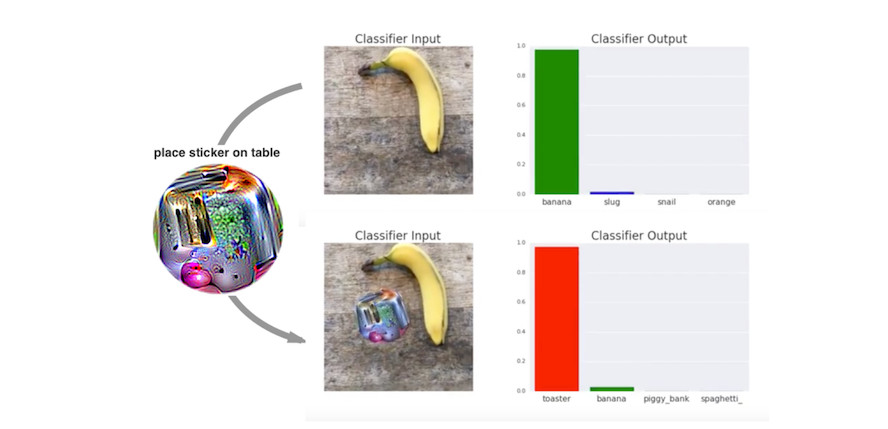
\includegraphics[scale=0.7]{images/adversarial-toaster.png}
	\label{fig:6_5}
	\caption{Một mảng làm cho mạng VGG16 huấn luyện trên tập ImageNet phân biệt ảnh quả chuối thành máy nướng bánh.}
\end{figure*}

Phương pháp này khác xa với các phương pháp khác cho các mẫu dữ liệu đối kháng, do ràng buộc rằng mẫu đối kháng phải rất gần với ảnh gốc được loại bỏ. Thay vào đó, phương pháp này hoàn toàn thay thế một phần của ảnh gốc với một mảng có hình dạng bất kỳ. Mảng được tối ưu trên các ảnh nền (background images) khác nhau, với vị trí khác nhau mảng trên ảnh nền (đôi lúc bị dịch, đôi lúc lại lớn hơn hay nhỏ hơn và bị xoay nên mảng hoạt động được trong nhiều tình huống khác nhau). Cuối cùng, hình ảnh tối ưu này có thể được in ra và sử dụng để đánh lừa các bộ phân loại hình ảnh trong thực tế.

\paragraph{Đừng bao giờ mang một con rùa in 3D đến một trận đấu súng, thậm chí cả khi máy tính của ta cho đó là một ý tưởng tuyệt vời: Các mẫu dữ liệu đối kháng linh hoạt}

Phương pháp tiếp theo về bản chất chỉ là ta thêm một thành phần vào trong mảng đối kháng. Athalye et al. (2017) đã in ra một con rùa 3D được thiết kế trông giống như một khẩu súng trường đối với mạng nơ-ron sâu khi nhìn từ  mọi góc cạnh. Đúng vậy, bạn đọc đúng rồi đấy. Một vật trông  giống như một con rùa đối với con người lại trông giống như một khẩu súng trường đối với máy tính!

\begin{figure*}[h!]
	\centering
	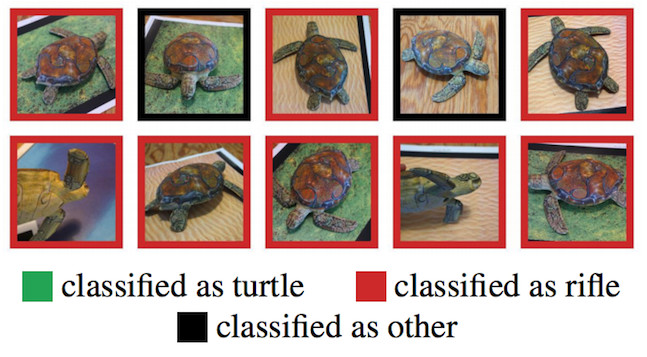
\includegraphics[scale=0.3]{images/adversarial-turtle.png}
	\label{fig:6_6}
	\caption{Athalye et al. (2017) đã tạo ra một vật in 3D được nhận diện trông giống như một khẩu súng bởi bộ phân loại InceptionV3 huấn luyện trên Tensorflow.}
\end{figure*}

Các tác giả đã tìm ra cách để tạo các mẫu đối kháng 3D cho các bộ phân loại làm việc trên ảnh 2D, đó là đối kháng dựa trên các biến đổi, ví dụ như xoay, phóng to... Các phương pháp khác như FGSM không hoạt động khi hình ảnh bị xoay hoặc hiển thị ở các góc khác nhau. Athalye et al. (2017) đề xuất thuật toán Expection Over Transformation (EOT), là một phương pháp sinh ra các mẫu dữ liệu đối kháng mà vẫn có thể hoạt động khi các hình ảnh bị biến đổi. Ý tưởng chính đằng sau EOT là tối ưu hóa các mẫu dữ liệu đối kháng qua nhiều biến đổi nhất có thể. Thay vì tối thiểu hóa khoảng cách giữa các mẫu dữ liệu đối kháng và hình ảnh gốc, EOT giữ cho khoảng cách kỳ vọng giữa hai mẫu này dưới một ngưỡng nhất định khi cho trước một phân phối của các biến đổi (distribution of possible transformations). Khoảng cách kỳ vọng theo biến đổi có thể được viết lại như sau:

\[\mathbb{E}_{t\sim{}T}[d(t(x^\prime),t(x))]\]

Trong đó $x$ là hình ảnh gốc, $t(x)$ là hình ảnh đã qua biến đổi (ví dụ: xoay), $x^\prime$ là mẫu dữ liệu đối kháng và $t(x^\prime)$ là phiên bản biến đổi của $x^\prime$. Bên cạnh làm việc với phân phối của các biến đổi, EOT cũng dùng các phương pháp tối ưu để tìm ra các mẫu dữ liệu đối kháng. Chúng ta cố gắng tìm một mẫu dữ liệu đối kháng $x^\prime$ mà cực đại hóa xác suất cho lớt $y_t$ (ví dụ: súng trường) trên toàn bộ phân phối của các biến đổi T có thể:

\[\arg\max_{x^\prime}\mathbb{E}_{t\sim{}T}[log{}P(y_t|t(x^\prime))]\]

Với ràng buộc rằng khoảng cách kỳ vọng trên toàn bộ biến đổi có thể giữa mẫu dữ liệu đối kháng $x^\prime$ và hình ảnh gốc $s$ duy trì ở dưới một ngưỡng nhất định. 

 \[\mathbb{E}_{t\sim{}T}[d(t(x^\prime),t(x))]<\epsilon\quad\text{and}\quad{}x\in[0,1]^d\]

Tôi nghĩ rằng ta nên cân nhắc phương pháp này. Các phương pháp khác dựa trên các biến đổi của hình ảnh kỹ thuật số. Tuy nhiên, những hình in 3D này, các mẫu dữ liệu đối kháng linh hoạt có thể được chèn vào bất cứ trường hợp thực tế nào và đánh lừa máy tính để phân loại sai đối tượng. Hãy để tôi chỉ ra vấn đề: Sẽ ra sao nếu ai đó tạo ra một khẩu súng nhưng lại giống như một con rùa?

\paragraph{Đối thủ bịt mắt (The blindfolded adversary): Tấn công hộp đen}

Hãy hình dung theo kịch bản sau: Tôi đưa cho bạn truy cập vào bộ phân loại tốt nhất của tôi thông qua Web API. Bạn có thể lấy các dự đoán từ mô hình, nhưng bạn không có quyền can thiệp vào các trọng số mô hình. Từ đó, bạn có thể gửi dữ liệu lên và mô hình của tôi trả về các kết quả tương ứng. Hầu hết các phương pháp tấn công dùng mẫu dữ liệu đối kháng không được thiết kế để hoạt động trong kịch bản này bởi vì chúng yêu cầu truy cập vào gradient của mạng nơ-ron sâu để tìm các mẫu dữ liệu đối kháng. Papernot et al. (2017) đã chỉ ra rằng nó hoàn toàn có thể tạo ra các mẫu dữ liệu đối kháng mà không cần thông tin bên trong của mô hình và không cần truy cập vào dữ liệu huấn luyện. Đây là kiểu tấn công vô thức (zero-knowledge), hay còn được gọi là tấn công hộp đen.

Nó làm việc như thế nào:

1. Bắt đầu với một vài hình ảnh nằm trong phân phối của dữ liệu huấn luyện. Ví dụ, nếu bộ phân loại đang bị tấn công là một bộ phân loại chữ số (từ 0 đến 9), ảnh được sử dụng cũng nên là các ảnh chữ số. Ta cần biết về miền dữ liệu huấn luyện, nhưng không cần thiết truy cập chúng.

2. Lấy dự đoán cho tập hình ảnh hiện tại từ mô hình hộp đen đó.

3. Huấn luyện một mô hình đại diện (surrogate model) trên tập dữ liệu ảnh hiện tại.

4. Tạo ra một tập dữ liệu ảnh nhân tạo mới bằng việc thay đổi các pixel trên các hình ảnh này để làm mô hình có phương sai lớn hơn (more variance).

5. Lặp lại các bước 2 đến 4 cho một số epochs nhất định.

6. Tạo ra các mẫu dữ liệu đối kháng từ mô hình đại diện sử dụng phương pháp FGSM (hoặc tương tự).

7. Tấn công mô hình ban đầu với các mẫu dữ liệu đối kháng.

Mục đích của mô hình đại diện là xấp xỉ ranh giới quyết định (decision boundaries) của mô hình hộp đen, nhưng không cần thiết đạt độ chính xác tương đương.

Các tác giả đã kiểm thử cách tiếp cạnh này bằng cách tấn công các bộ phân loại được huấn luyện trên một số dịch vụ học máy đám mây (cloud machine learning services). Những dịch vụ này huấn luyện bộ phân loại hình ảnh trên dữ liệu và nhãn mà người dùng tải lên. Phần mềm huấn luyện mô hình tự động, đôi khi bằng một thuật toán mà người dùng không biết và triển khai nó. Bộ phân loại có thể cho các dự đoán cho các hình ảnh được đăng tải lên, nhưng chính mô hình đó lại không thể được kiểm soát hoặc tải về. Các tác giả đã tìm ra các mẫu dữ liệu đối kháng cho rất nhiều mô hình kiểu đám mây, và lên đến 84\% các mẫu dữ liệu đối kháng được phân loại sai lớp.

Phương pháp trên thậm chí làm việc cả khi mô hình hộp đen không phải là một mạng nơ-ron. Chúng bao hàm những mô hình học máy mà không có gradient ví dụ như cây quyết định.

\subsection{Góc nhìn bảo mật an ninh}

Học máy xử lý vấn đề: Dự đoán các điểm dữ liệu mới từ một phân phối đã biết. Hệ thống phòng thủ trước các tấn công đối kháng xử lý vấn đề: Dự đoán một cách linh hoạt các điểm dữ liệu mới từ một phân phối chưa biết của các đầu vào đối kháng (adversarial inputs). Vì học máy được tích hợp vào càng nhiều hệ thống, như xe tự hành hay thiết bị y tế, nên chúng cũng đang là các trọng điểm của các cuộc tấn công. Thậm chí nếu các dự đoán của mô hình học máy trên tập dữ liệu kiểm thử là chính xác 100\%, thì các mẫu dữ liệu đối kháng vẫn có thể được tìm thấy để đánh lừa mô hình. Việc bảo vệ các mô hình học máy chống lại các cuộc tấn công mạng là một lĩnh vực mới của an ninh mạng.

Biggio et. at (2018) đã nhận xét về học máy đối kháng (adversarial machine learning), và phần này sẽ thảo luận về nhận xét đó. An ninh mạng là một cuộc chạy đua vũ trang mà người tấn và kẻ phòng thủ đánh lừa nhau hết lần này đến lần khác.

\textbf{Có ba nguyên tắc vàng trong an ninh mạng: 1) Biết về đối thủ của bạn 2) Chủ động và 3) Tự bảo vệ chính mình.}

Các ứng dụng khác nhau có các đối thủ khác nhau. Những kẻ cố gắng lừa gạt người khác qua email để lấy tiền của họ là đối của người dùng và nhà cung cấp dịch vụ email. Những người cung cấp dịch vụ muốn bảo vệ người dùng của họ, để họ tiếp tục sử dụng dịch vụ mail, những kẻ tấn công thì muốn người khác đưa chúng tiền. Hiểu về các bất lợi bạn gặp phải nghĩa là biết về mục đích của chúng. Giả sử rằng bạn không biết các thư rác đó tồn tại và phiền hà duy nhất gặp phải chỉ là việc chúng lạm dụng dịch vụ email để gửi các bản nhạc lậu, thì hệ thống phòng thủ sẽ phải khác đi (ví dụ: quét các tệp đính kèm để xem xét bản quyền thay vì phân tích văn bản).

Tính chủ động nghĩa là chủ động kiểm thử và xác định các điểm yếu có trong hệ thống. Bạn chủ động khi tự đánh lừa mô hình với các mẫu dữ liệu đối kháng và sau đó phòng thủ chống lại chúng. Sử dụng phương pháp diễn dịch để hiểu các đặc trưng  quan trọng và ảnh hưởng của chúng đến việc dự đoán cũng là một bước chủ động trong việc hiểu các điểm yếu của các mô hình học máy. Là một nhà khoa học dữ liệu, bạn có tin vào mô hình của bạn trong thế giới đầy nguy hiểm mà không viễn kiến vào năng lực dự đoán trên tập dữ liệu kiểm thử? Bạn đã từng phân tích mô hình hành xử như thế nào trong các kịch bản khác nhau, xác định đầu vào nào là quan trọng nhất, kiểm tra các giải thích cho dự đoán trên một số mẫu dữ liệu? Bạn đã thử tìm qua các đầu vào đối kháng? Khả năng diễn giải của các mô hình học máy đóng một vai trò chính trong an ninh mạng. Tính thụ động, đối lập với chủ động, nghĩa rằng chờ cho hệ thống bị tấn công và hiểu ra vấn đề sau đó lập hệ thống phòng thủ.

Vậy làm sao chúng ta bảo vệ các hệ thống học máy chống lại các mẫu dữ liệu đối kháng? Một phương pháp chủ động là liên tục lặp lại huấn luyện các bộ phân loại với các mẫu dữ liệu đối kháng, hay được gọi là huấn luyện đối kháng. Các phương pháp tiếp cận khác dựa trên lý thuyết trò chơi (game theory), ví dụ như học các phép biến đổi bất biến của các đặc trưng hoặc tối ưu một cách linh động - robust optimization (qua điều chuẩn). Các phương pháp khác sử dụng nhiều bộ phân loại thay vì chỉ một và cho chúng bỏ phiếu dự đoán (ensemble), nhưng không có gì để đảm bảo, vì chúng có thể chịu các tấn công từ các mẫu dữ liệu đối kháng tương tự. Một phương pháp khác không hoạt động tốt đó là loại bỏ gradient (gradient masking) - xây dựng mô hình không dùng các gradient bằng cách sử dụng một bộ phân loại lân cận gần nhất thay vì sử dụng mô hình gốc.

Chúng ta có thể phân biệt các loại tấn công bằng cách xác định kẻ tấn công biết bao nhiêu về hệ thống. Các kẻ tấn công có thể có kiến thức toàn bộ (tấn công hộp trắng), nghĩa là chúng biết tất cả mọi thứ về mô hình như loại mô hình, các tham số và dữ liệu huấn luyện; kẻ tấn công có thể có một phần kiến thức (tấn công hộp xám), nghĩa là chúng chỉ có thể biết về biểu diễn và loại mô hình mà đã sử dụng, nhưng không thể truy cập và dữ liệu huấn luyện hay các tham số mô hình; kẻ tấn công có thể không hề có kiến thức gì (tấn công hộp đen), nghĩa rằng chúng chỉ truy vấn mô hình và không truy cập vào dữ liệu huấn luyện hoặc thông tin của các tham số mô hình. Phụ thuộc và cấp bậc thông tin, kẻ tấn công có thể sử dụng các kỹ thuật khác nhau để tấn công mô hình. Vì chúng ta đã thấy trong các mẫu dữ liệu, thậm chí trong trường hợp hộp đen, các mẫu dữ liệu đối kháng có thể được tạo ra, vì vậy việc giấu đi thông tin về dữ liệu và mô hình là không đủ để phòng thủ lại các cuộc tấn công.

Với bản chất của trò chơi ``mèo vờn chuột'' giữa kẻ tấn công và người phòng thủ, chúng ta sẽ chứng kiến nhiều sự phát triển và đổi mới trong lĩnh vực này. Hãy tưởng tượng có bao nhiêu loại email rác mới được sinh ra hàng ngày. Các phương pháp mới cho việc tấn công các mô hình học máy được phát minh ra thì lại có các biện pháp phòng thủ để chống lại chúng. Nhiều phương pháp tấn công mạnh mẽ được phát triển để trốn tránh hệ thống phòng thủ cuối cùng, vân vân và sẽ không có hồi kết. Với chương này tôi mong rằng có thể giúp bạn có cái nhìn nhạy bén hơn về các vấn đề của dữ liệu đối kháng và vì chỉ khi có tính chủ động nghiên cứu về các mô hình học máy, chúng ta mới có thể khám phá và khắc phục được các điểm yếu của các mô hình học máy.
\clearpage
\section{Nguyên mẫu và ngoại lai - Prototypes and criticisms}

Nguyên mẫu là một cá thể dữ liệu đại diện cho cả tập dữ liệu. Ngoại lai là một điểm dữ liệu không được bao hàm (không cùng phân phối dữ liệu với) bởi tập hợp các nguyên mẫu. Mục đích sử dụng của ngoại lai là cung cấp những hiểu biết sâu sắc về tập dữ liệu cùng với các nguyên mẫu, đặc biệt là đối với các điểm dữ liệu mà nguyên mẫu không thể thể hiện. Các nguyên mẫu và ngoại lai có thể được sử dụng độc lập với mô hình học máy để mô tả dữ liệu, nhưng chúng cũng có thể được sử dụng để tạo mô hình khả diễn giải nội tại (intrinsically interpretable) được hoặc để làm cho mô hình hộp đen trở nên khả diễn giải.

Trong chương này, ta sử dụng cụm từ ``điểm dữ liệu'' để chỉ một mẫu dữ liệu duy nhất, và để nhấn mạnh cách giải thích rằng một mẫu dữ liệu cũng là một điểm trong hệ tọa độ đa chiều mà mỗi đặc trưng là một chiều. Hình sau đây cho thấy một phân phối dữ liệu mô phỏng, với một số trường hợp được chọn làm nguyên mẫu và một số trường hợp là ngoại lai. Những điểm nhỏ là dữ liệu, những điểm lớn là ngoại lai và những ô vuông lớn là những nguyên mẫu. Các nguyên mẫu được chọn (theo cách thủ công) để bao phủ các trung tâm của các cụm dữ liệu và các ngoại lai là các điểm trong các cụm không xuất hiện nguyên mẫu. Các nguyên mẫu và ngoại lai luôn là các mẫu dữ liệu thực tế từ tập dữ liệu.


\begin{figure*}[h!]
	\centering
	\includegraphics[scale=0.2]{images/unnamed-chunk-43-1.png}
	\label{fig:6_7}
	\caption{Nguyên mẫu và ngoại lai cho một phân phối dữ liệu với hai đặc trưng x1 và x2.}
\end{figure*}

Ở đây tôi chọn các nguyên mẫu theo cách thủ công, do đó kết quả có thể không được tốt. Có nhiều cách tiếp cận để tìm ra nguyên mẫu trong dữ liệu. Một trong số đó là k-medoids, một thuật toán phân cụm liên quan đến thuật toán k-means. Bất kỳ thuật toán phân cụm nào trả về các điểm dữ liệu thực tế dưới dạng trung tâm cụm sẽ thỏa mãn cho việc chọn các nguyên mẫu. Nhưng hầu hết các phương pháp này chỉ tìm thấy nguyên mẫu chứ không trả về ngoại lai. Chương này trình bày thuật toán MMD-critic của Kim et. al (2016), là một cách tiếp cận kết hợp việc tìm ra các nguyên mẫu và ngoại lai một các đồng thời

MMD-critic so sánh phân phối dữ liệu thực tế và sự phân bố của các nguyên mẫu đã chọn. Đây là khái niệm trung tâm cho việc hiểu phương pháp này. MMD-critic chọn các nguyên mẫu giúp giảm thiểu sựsai khác giữa hai phân phối đã nêu. Các điểm dữ liệu trong các cụm có mật độ cao là các nguyên mẫu tốt, đặc biệt khi các điểm được chọn từ các ``cụm dữ liệu'' khác nhau. Các điểm dữ liệu từ các cụm không được giải thích rõ bởi các nguyên mẫu được chọn làm ngoại lai.

Chúng ta hãy nghiên cứu sâu hơn về lý thuyết.

\subsection{Lý thuyết}

MMD-critic có thể được tóm tắt ngắn gọn như sau:

1. Chọn số lượng nguyên mẫu và ngoại lai bạn muốn tìm.

2. Tìm nguyên mẫu bằng tìm kiếm tham lam (greedy search). Các nguyên mẫu được chọn sao cho phân phối của các nguyên mẫu gần với phân phối dữ liệu.

3. Tìm ngoại lai bằng cách tìm kiếm tham lam. Các điểm được chọn làm ngoại lai nằm trong cụm có phân phối của các nguyên mẫu khác với phân phối của dữ liệu.

Chúng tôi cần một vài công cụ để tìm nguyên mẫu và ngoại lai cho tập dữ liệu với MMD-critic. Cơ bản nhất, chúng ta cần một hàm nhân để ước tính mật độ dữ liệu. Kernel là một hàm gán trọng số cho hai điểm dữ liệu theo khoảng cách (proximity) của chúng. Dựa trên ước tính mật độ, ta cần một thước đo cho ta biết hai phân phối khác nhau như thế nào để ta có thể xác định xem liệu phân phối của các nguyên mẫu mà ta chọn có gần với phân phối dữ liệu hay không. Điều này được giải quyết bằng cách đo sự khác biệt trung bình tối đa (maximum mean discrepancy - MMD). Cũng dựa trên hàm nhân, chúng ta cần hàm nhân chứng (witness function) để cho chúng ta biết hai phân phối khác nhau như thế nào tại một điểm dữ liệu cụ thể. Với hàm nhân chứng, chúng ta có thể chọn các ngoại lai, tức là các điểm dữ liệu mà tại đó phân phối của các nguyên mẫu và dữ liệu khác nhau và hàm nhân chứng nhận các giá trị tuyệt đối lớn. Cuối cùng, ta cần một phương pháp tìm kiếm các nguyên mẫu và ngoại lai tốt, vấn đề này được giải quyết bằng một thuật toán tìm kiếm tham lam đơn giản.

Chúng ta hãy bắt đầu với khác biệt trung bình tối đa (MMD), công thức này đo lường sự khác biệt giữa hai phân phối. Việc lựa chọn các nguyên mẫu tạo ra sự phân bố mật độ của các nguyên mẫu. Ta muốn đánh giá xem phân phối nguyên mẫu có khác với phân phối dữ liệu hay không. Do đó, ta ước tính cả hai phân phối với các hàm mật độ nhân. MMD đo lường sự khác biệt giữa hai phân phối, trên một không gian hàm của sự khác biệt giữa các kỳ vọng theo hai phân phối. Tất cả rõ ràng chứ? Cá nhân tôi hiểu những khái niệm này tốt hơn nhiều khi tôi quan sát tính toán với dữ liệu cụ thể. Công thức sau đây cho biết cách tính MMD bình phương (MMD2):

$$MMD^2=\frac{1}{m^2}\sum_{i,j=1}^m{}k(z_i,z_j)-\frac{2}{mn}\sum_{i,j=1}^{m,n}k(z_i,x_j)+\frac{1}{n^2}\sum_{i,j=1}^n{}k(x_i,x_j)$$

$k$ là một hàm nhân đo sự giống nhau của hai điểm, ta sẽ nói thêm về điều này sau. $m$ là số nguyên mẫu $z$ và $n$ là số điểm dữ liệu $x$ trong tập dữ liệu ban đầu của chúng ta. Nguyên mẫu $z$ là sự lựa chọn từ các điểm dữ liệu $x$. Mỗi điểm là đa chiều, tức là nó có thể có nhiều đặc trưng. Mục tiêu của MMD-critic là giảm thiểu MMD2. MMD2 càng gần bằng 0, phân phối của các nguyên mẫu càng khớ với dữ liệu. Chìa khóa để đưa MMD2 xuống 0 là thành phần ở giữa trong công thức trên, tính toán khoảng cách trung bình giữa các nguyên mẫu và tất cả các điểm dữ liệu khác (nhân với 2). Nếu thành phần này cộng với thành phần đầu tiên (khoảng cách trung bình của các nguyên mẫu với nhau) cộng với thành phần cuối cùng (khoảng cách trung bình của các điểm dữ liệu với nhau), thì nguyên mẫu sẽ giải thích dữ liệu một cách hoàn hảo. Hãy thử xem điều gì sẽ xảy ra với công thức trên nếu ta sử dụng tất cả $n$ điểm dữ liệu làm nguyên mẫu.

Hình ảnh sau đây minh họa cách tính MMD2. Hình đầu tiên hiển thị các điểm dữ liệu với hai đặc trưng, theo đó ước tính mật độ dữ liệu được hiển thị với nền bóng mờ. Mỗi hình còn lại là các lựa chọn nguyên mẫu khác nhau, cùng với giá trị MMD2. Nguyên mẫu là các chấm lớn và phân bố của chúng được thể hiện dưới dạng các đường đồng mức (contour lines). Việc lựa chọn các nguyên mẫu mà phủ dữ liệu một cách tốt nhất (dưới cùng bên trái) cho ta giá trị sai khác nhỏ nhất.

\begin{figure*}[h!]
	\centering
	\includegraphics[scale=0.2]{images/mmd-1.png}
    \caption{Giá trị MMD2 cho một tập dữ liệu với hai đặc trưng và các cách lựa chọn nguyên mẫu khác nhau.}
\end{figure*}

Hàm nhân có thể là hàm nhân xuyên tâm cơ sở:

$$k(x,x^\prime)=exp\left(-\gamma||x-x^\prime||^2\right)$$

trong đó $||x-x^\prime||^2$ là khoảng cách Euclidean giữa hai điểm và $\gamma$ là thông số mở rộng (scaling parameter). Giá trị của nhân giảm theo khoảng cách giữa hai điểm và nằm trong khoảng 0 và 1: 0 khi hai điểm xa nhau vô cực và 1 khi hai điểm trùng nhau.

Ta gói gọn cách tính MMD2, nhân và tìm kiếm tham lam vào một thuật toán để tìm nguyên mẫu:

1. Bắt đầu với một danh sách rỗng các nguyên mẫu.

2. Khi số lượng nguyên mẫu thấp hơn số m đã chọn:

- Đối với mỗi điểm trong tập dữ liệu, kiểm tra xem MMD2 bị giảm bao nhiêu khi điểm đó được thêm vào danh sách các nguyên mẫu. Thêm điểm dữ liệu mà làm giảm MMD2 vào danh sách.

3. Trả về danh sách các nguyên mẫu.

Để tìm ngoại lai ta cần hàm nhân chứng, cho ta biết hai phân phối khác nhau như thế nào tại một điểm cụ thể. Giá trị này được tính như sau:

$$witness(x)=\frac{1}{n}\sum_{i=1}^nk(x,x_i)-\frac{1}{m}\sum_{j=1}^mk(x,z_j)$$

Đối với hai tập dữ liệu (có các đặc trưng giống nhau), hàm nhân chứng cung cấp cho ta phương tiện đánh giá xem điểm x khớp hơn với phân phối thực nghiệm nào. Để tìm ra các ngoại lai, ta tìm kiếm các giá trị cực trị của hàm nhân chứng theo cả chiều âm và chiều dương. Số hạng đầu tiên trong hàm nhân chứng là khoảng cách trung bình giữa điểm x và dữ liệu, tương ứng, số hạng thứ hai là khoảng cách trung bình giữa điểm x và các nguyên mẫu. Nếu hàm nhân chứng cho một điểm x gần bằng 0, thì hàm mật độ của dữ liệu và các nguyên mẫu gần nhau, có nghĩa là phân phối của các nguyên mẫu giống với phân phối của dữ liệu tại điểm x. Hàm nhân chứng nhận giá trị âm tại điểm x có nghĩa là phân phối nguyên mẫu quá ước lượng (overestimate) phân phối dữ liệu (ví dụ: nếu chúng ta chọn một nguyên mẫu nhưng chỉ có vài điểm dữ liệu gần đó); một hàm nhân chứng là dương tại điểm x có nghĩa là phân phối nguyên mẫu dưới ước lượng (underestimate) phân phối dữ liệu (ví dụ: nếu có nhiều điểm dữ liệu xung quanh x nhưng ta chưa chọn bất kỳ nguyên mẫu nào gần đó). Để cho bạn dễ hiểu, ta sử dụng lại các nguyên mẫu từ hình ảnh trước đó với MMD2 thấp nhất và hiển thị hàm nhân chứng cho một vài điểm được chọn thủ công. Các nhãn trong biểu đồ sau đây hiển thị giá trị của hàm nhân chứng cho các điểm khác nhau được đánh dấu là hình tam giác. Chỉ có điểm ở giữa có giá trị tuyệt đối cao và do đó là ứng cử viên sáng giá cho một ngoại lai.

\begin{figure*}[h!]
	\centering
	\includegraphics[scale=0.2]{images/witness-1.png}
    \caption{Giá trị của hàm nhân chứng tại các điểm khác nhau.}
\end{figure*}

Hàm nhân chứng cho phép ta tìm kiếm một cách tường minh các mẫu dữ liệu không được thể hiện tốt bởi các nguyên mẫu. Ngoại lai là những điểm có giá trị tuyệt đối cao trong hàm nhân chứng. Giống như nguyên mẫu, các ngoại lai cũng được tìm thấy thông qua việc tìm kiếm tham lam. Nhưng thay vì giảm MMD2, ta đang tìm kiếm các điểm tối đa hóa hàm chi phí bao gồm hàm nhân chứng và thông số điều chuẩn. Thanh phần được bổ sung trong hàm tối ưu hóa làm tăng tính đa dạng của các điểm, điều này cần thiết để các điểm đến từ các cụm dữ liệu khác nhau.

Bước thứ hai độc lập với cách các nguyên mẫu được tìm ra. Ta cũng có thể chọn thủ công một số nguyên mẫu và sử dụng quy trình được mô tả ở trên để tìm ra các ngoại lai. Hoặc các nguyên mẫu có thể được tìm ra từ bất kỳ thuật toán phân cụm nào, như k-medoid.

Trên đây là các phần quan trọng về lý thuyết của MMD-critic. Vẫn còn một câu hỏi: \textbf{Làm cách nào ta có thể áp dụng MMD-critic trong học máy khả diễn giải?}

MMD-critic có thể bổ sung tính diễn giải theo ba cách: Bằng cách giúp hiểu rõ hơn về phân phối dữ liệu; bằng cách xây dựng một mô hình khả diễn giải; bằng cách làm cho mô hình hộp đen trở nên khả diễn giải.

Nếu bạn áp dụng MMD-critic vào phân tích dữ liệu để tìm nguyên mẫu và ngoại lai, nó sẽ giúp bạn tăng thêm hiểu biết về dữ liệu bạn đang có, đặc biệt nếu bạn có một phân phối dữ liệu phức tạp với nhiều nhiễu. Với MMD-critic bạn có thể đạt được nhiều hơn thế!

Ví dụ: ta có thể tạo một mô hình dự đoán khải diễn giải: gọi là ``mô hình nguyên mẫu gần nhất''. Chức năng dự đoán được định nghĩa là:

$$\hat{f}(x)=argmax_{i\in{}S}k(x,x_i)$$

có nghĩa là chúng ta chọn nguyên mẫu $i$ từ tập các nguyên mẫu $S$ gần nhất với điểm dữ liệu mới, trả về giá trị cao nhất cho hàm nhân. Bản thân nguyên mẫu được trả về như một lời giải thích cho dự đoán. Quy trình này có ba tham số: Loại nhân, tham số mở rộng nhân và số lượng nguyên mẫu. Tất cả các tham số có thể được tối ưu hóa trong bước kiểm định chéo (cross validation). Ngoại lai không được dùng trong trường hợp này.

Hoặc ta có thể sử dụng MMD-critic để biến bất kỳ mô hình học máy nào cũng trở nên khả diễn giải một cách toàn tục bằng cách kiểm tra các nguyên mẫu và ngoại lai cùng với các dự đoán của mô hình. Quy trình như sau:

1. Tìm nguyên mẫu và ngoại lai với MMD-critic.

2. Huấn luyện mô hình học máy như bình thường.

3. Dự đoán đầu ra cho các nguyên mẫu và ngoại lai với mô hình học máy.

4. Phân tích dự đoán: Thuật toán sai trong những trường hợp nào? Giờ ta đã có một số mẫu dữ liệu đại diện cho tập dữ liệu và giúp ta tìm ra điểm yếu của mô hình học máy.

Vậy chúng có ích như thế nào? Hãy nhớ lại khi bộ phân loại hình ảnh của Google xác định người da đen là khỉ đột! Có lẽ họ nên sử dụng quy trình được mô tả ở đây trước khi triển khai mô hình nhận dạng hình ảnh của họ. Chỉ kiểm tra hiệu suất của mô hình thôi là chưa đủ, bởi vì nếu nó đúng 99\%, vấn đề này vẫn có thể nằm trong 1\% còn lại. Và nhãn cũng có thể sai! Xem qua tất cả dữ liệu huấn luyện và thực hiện kiểm tra nhanh có thể chỉ ra vấn đề, nhưng sẽ không khả thi. Nhưng việc lựa chọn - giả sử vài nghìn - nguyên mẫu và ngoại lai là khả thi thì ta có thể nhìn ra vấn đề của dữ liệu: Nó có thể cho ta biết dữ liệu thiếu hình ảnh của những người có làn da sẫm màu, điều này tương đương với việc thiếu sự đa dạng trong tập dữ liệu. Hoặc MMD-critic có thể hiển thị một hoặc nhiều hình ảnh của một người có làn da đen như một nguyên mẫu hoặc (có thể) như một ngoại lai với cụm ``khỉ đột''. Tôi không chắc chắn tuyệt đối rằng MMD-critic sẽ giúp ngăn chặn những sai lầm kiểu này, nhưng đây là một phép kiểm thử đúng đắn.

\subsection{Ví dụ}
Ví dụ sau về MMD-critic sử dụng tập dữ liệu chữ số viết tay.

Nhìn vào các nguyên mẫu thực tế, bạn có thể nhận thấy rằng số lượng hình ảnh trên mỗi chữ số là khác nhau. Điều này là do nguyên mẫu đã được tìm kiếm trên toàn bộ tập dữ liệu chứ không phải ta xác định trước số lượng số cố định cho mỗi lớp. Đúng như dự đoán, các nguyên mẫu cho thấy các cách viết chữ số khác nhau.
\begin{figure*}[h!]
	\centering
	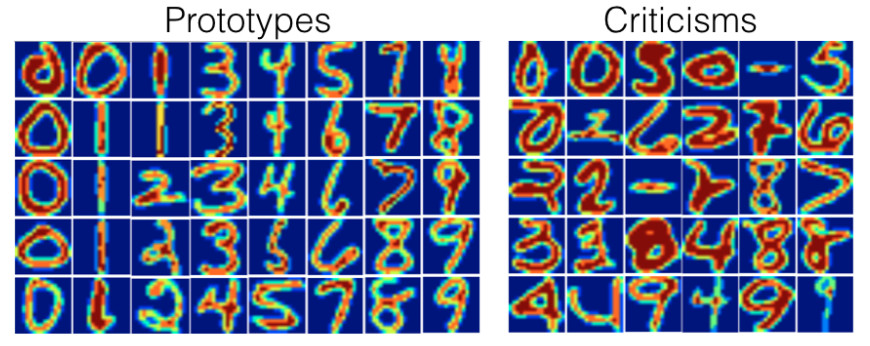
\includegraphics[scale=0.7]{images/proto-critique2.jpg}
    \caption{Nguyên mẫu cho tập dữ liệu chữ số viết tay.}
\end{figure*}
\subsection{Ưu điểm}
Trong một nghiên cứu người dùng, các tác giả của MMD-critic đã đưa các hình ảnh cho những người tham gia, họ phải so sánh trực quan với một trong hai bộ hình ảnh, mỗi bộ đại diện cho một trong hai lớp (ví dụ: hai giống chó). \textbf{Những người tham gia thực hiện tốt nhất khi các bộ hiển thị nguyên mẫu và ngoại lai} thay vì hình ảnh ngẫu nhiên của một lớp.

Bạn có thể tự do \textbf{lựa chọn số lượng nguyên mẫu và ngoại lai}.

MMD-critic làm việc trên các ước lượng mật độ (density estimate) của dữ liệu. Do đó, phương pháp sẽ này\textbf{ hoạt động với bất kỳ loại dữ liệu nào và bất kỳ loại mô hình học máy nào}.
 
Thuật toán \textbf{dễ dàng cho việc lập trình}
 
MMD-critic rất linh hoạt trong cách sử dụng để tăng khả năng diễn giải. Nó có thể được sử dụng để hiểu các phân phối dữ liệu phức tạp. Nó có thể được sử dụng để xây dựng một mô hình học máy khả giải thích. Hoặc nó có thể làm sáng tỏ việc ra quyết định của một mô hình hộp đen.

\textbf{Việc tìm kiếm ngoại lai độc lập với quá trình lựa chọn nguyên mẫu.} Nhưng sẽ hợp lý nếu chọn nguyên mẫu theo MMD-critic, vì cả nguyên mẫu và ngoại lai đều được tạo ra bằng cách sử dụng cùng một phương pháp.

\subsection{Nhược điểm}
Mặc dù, về mặt toán học, nguyên mẫu và ngoại lai được định nghĩa khác nhau, nhưng \textbf{sự phân biệt của chúng lại dựa trên giá trị giới hạn (cut-off value)} (số lượng nguyên mẫu). Giả sử bạn chọn số lượng nguyên mẫu quá thấp để bao phủ phân phối dữ liệu, ngoại lai sẽ nằm ở những khu vực không được giải thích rõ ràng. Nhưng nếu bạn thêm nhiều nguyên mẫu hơn, chúng cũng sẽ nằm ở cùng khu vực. Bất kỳ diễn giải nào cũng phải tính đến rằng ngoại lai phụ thuộc mạnh mẽ vào các nguyên mẫu hiện có và giá trị giới hạn (tùy ý) cho số lượng nguyên mẫu.

Bạn phải \textbf{chọn số lượng nguyên mẫu và ngoại lai}. Càng nhiều càng tốt tuy nhiên nó cũng là một bất lợi. Chúng ta thực sự cần bao nhiêu nguyên mẫu và ngoại lai? Càng nhiều càng tốt? Càng ít càng tốt? Một giải pháp là chọn số lượng nguyên mẫu và ngoại lai bằng cách đo lượng thời gian con người có, điều này sẽ phụ thuộc vào ứng dụng cụ thể. Chỉ khi sử dụng MMD-critic để xây dựng bộ phân loại, ta mới có cách tối ưu hóa trực tiếp. Một giải pháp có thể là hiển thị số lượng nguyên mẫu trên trục x và ước lượng MMD2 trên trục y. Chúng ta sẽ chọn số lượng nguyên mẫu nơi đường MMD2 bị làm phẳng.

Các tham số khác là cách chọn nhân (kernel) và tham số mở rộng nhân. Ta có cùng một vấn đề với số lượng nguyên mẫu và ngoại lai: \textbf{Làm thế nào để ta có thể chọn một nhân và tham số mở rộng}? Một lần nữa, khi chúng ta sử dụng MMD-critic, chúng ta có thể điều chỉnh các tham số nhân. Tuy nhiên, đối với các trường hợp sử dụng không được giám sát của MMD-critic (sử dụng tự động), việc này rõ ràng là hạn chế. (Có lẽ tôi hơi khắt khe ở đây, vì tất cả các phương pháp không được giám sát đều có vấn đề này).

Phương pháp này lấy tất cả các đặc trưng làm đầu vào, \textbf{bỏ qua thực tế là một số đặc trưng có thể không liên quan} để dự đoán kết quả. Một giải pháp là chỉ sử dụng các đặc trưng có liên quan, ví dụ như sử dụng các hình ảnh đã mã hóa thay vì các pixel gốc. Phương pháp này sẽ hoạt động tốt miễn là ta có thể ánh xạ dữ liệu gốc tới dạng dữ liệu mà ta đang dùng (chỉ chứa các đặc trưng có liên quan).

Có một số mã có sẵn cho MMD-critic, nhưng chúng \textbf{chưa được đóng gói và tài liệu hóa 1 cách tốt nhất}.

\subsection{Code và các phương pháp khác}
Code của MMD-critic do tác giả viết có thể tìm thấy ở \href{https://github.com/BeenKim/MMD-critic}{đây}.

Phương pháp đơn giản nhất để tìm nguyên mẫu đó là k-medoids bởi Kaufman et. al (1987).
\clearpage

\section{Các mẫu dữ liệu có ảnh hưởng}

Mô hình học máy là sản phẩm của dữ liệu huấn luyện và việc xóa một trong các mẫu dữ liệu huấn luyện có thể ảnh hưởng đến mô hình cuối cùng. Ta gọi một mẫu dữ liệu huấn luyện là ``có ảnh hưởng'' khi việc xóa nó khỏi dữ liệu huấn luyện làm thay đổi đáng kể các tham số hoặc dự đoán của mô hình. Bằng cách xác định các mẫu dữ liệu huấn luyện có ảnh hưởng, ta có thể ``gỡ lỗi'' các mô hình học máy và giải thích tốt hơn các hành vi và dự đoán của chúng.

Chương này chỉ cho ta hai phương pháp để xác định các mẫu dữ liệu có ảnh hưởng, đó là chẩn đoán xóa (deletion diagnostics) và hàm ảnh hưởng(influence functions). Cả hai phương pháp đều dựa trên thống kê linh động (robust statistics), điều này giúp các phương pháp thống kê ít bị ảnh hưởng bởi các giá trị ngoại lai hay các vi phạm về giả định của mô hình. Thống kê linh động cũng cung cấp các phương pháp để đo lường độ linh động của các ước lượng từ dữ liệu (chẳng hạn như ước lượng trung bình hay trọng số của mô hình).

Hãy tưởng tượng bạn muốn ước lượng thu nhập trung bình của người dân trong thành phố của bạn và hỏi mười người ngẫu nhiên trên đường phố họ kiếm được bao nhiêu. Ngoài thực tế là mẫu dữ liệu có thể có chất lượng kém, ước lượng thu nhập trung bình của bạn có thể bị ảnh hưởng bao nhiêu bởi một người? Để trả lời câu hỏi này, bạn có thể tính toán lại giá trị trung bình bằng cách bỏ qua các mẫu đơn lẻ hoặc suy ra bằng toán học thông qua ``hàm ảnh hưởng'' lượng giá trị trung bình có thể bị ảnh hưởng khi loại bỏ các mẫu đơn lẻ đó. Với phương pháp xóa, ta tính toán lại giá trị trung bình mười lần, mỗi lần bỏ qua một trong các báo cáo thu nhập và đo lường mức độ thay đổi ước lượng trung bình. Một sự thay đổi lớn có nghĩa là một mẫu dữ liệu có ảnh hưởng rất lớn. phương pháp thứ hai làm tăng trọng số của một người bằng một trọng số nhỏ nhất định, tương ứng với việc tính toán đạo hàm bậc nhất của một thống kê hoặc mô hình. phương pháp này còn được gọi là ``phương pháp vô cực'' hoặc ``hàm ảnh hưởng''. Nhân tiện, câu trả lời là ước lượng trung bình của bạn có thể bị ảnh hưởng rất mạnh bởi một mẫu duy nhất, vì giá trị trung bình tỷ lệ tuyến tính với các giá trị đơn lẻ. Một cách lựa chọn tốt hơn là sử dụng giá trị trung vị (median - giá trị mà tại đó một nửa số người kiếm được nhiều hơn và nửa còn lại ít hơn), bởi vì ngay cả khi người có thu nhập cao nhất trong mẫu của bạn kiếm được nhiều hơn mười lần trung vị, giá trị trung vị sẽ không bị thay đổi.

Chẩn đoán xóa và hàm ảnh hưởng cũng có thể được áp dụng cho các tham số hoặc dự đoán của mô hình học máy để hiểu hành vi của chúng tốt hơn hoặc để giải thích các dự đoán riêng lẻ. Trước khi xem xét hai phương pháp này để tìm các mẫu dữ liệu có ảnh hưởng, chúng ta sẽ xem xét sự khác biệt giữa một mẫu dữ liệu ngoại lai và một mẫu dữ liệu có ảnh hưởng.

\paragraph{Ngoại lai}

Một mẫu dữ liệu ngoại lai là một mẫu dữ liệu khác xa với các mẫu dữ liệu khác trong tập dữ liệu. ``Xa'' có nghĩa là khoảng cách, ví dụ khoảng cách Euclide, đến tất cả các mẫu dữ liệu khác là rất lớn. Trong một tập dữ liệu về trẻ sơ sinh, một trẻ sơ sinh nặng 6 kg sẽ được coi là một ngoại lai. Trong tập dữ liệu các tài khoản ngân hàng chủ yếu là tài khoản séc, một tài khoản cho vay chuyên dụng (số dư âm lớn, ít giao dịch) sẽ được coi là ngoại lai. Hình sau đây cho thấy ngoại lai của phân phối 1 chiều.

\begin{figure}[h!]
    \centering
    \includegraphics[scale=0.2]{images/outlier-1.png}
    \label{fig:6_11}
    \caption{Đặc trưng x tuân theo phân phối Gaussian với ngoại lai ở x=8.}
\end{figure}

Ngoại lai có thể là những điểm dữ liệu thú vị. Khi một ngoại lai ảnh hưởng đến mô hình, nó cũng là một mẫu có ảnh hưởng.

\paragraph{Mẫu dữ liệu có ảnh hưởng}

Một mẫu có ảnh hưởng là một mẫu dữ liệu mà việc loại bỏ nó có ảnh hưởng mạnh đến mô hình được huấn luyện. Các tham số hoặc dự đoán của mô hình càng thay đổi khi mô hình được huấn luyện lại với một mẫu cụ thể bị xóa khỏi dữ liệu huấn luyện, thì mẫu đó càng có ảnh hưởng. Việc một mẫu có ảnh hưởng đối với một mô hình được huấn luyện hay không cũng phụ thuộc vào giá trị của nó đối với mục tiêu $y$. Hình dưới đây cho thấy một mẫu có ảnh hưởng đối với mô hình hồi quy tuyến tính.

\begin{figure}[h!]
    \centering
    \includegraphics[scale=0.2]{images/influential-point-1.png}
    \caption{Một mô hình tuyến tính với một đặc trưng. Được huấn luyện lần đầu với dữ liệu đầy đủ và lần sau không có mẫu dữ liệu có ảnh hưởng. Việc loại bỏ mẫu dữ liệu có ảnh hưởng sẽ thay đổi đáng kể gradient(trọng số/hệ số)}
    \label{fig:6_12}
\end{figure}

\paragraph{Tại sao các mẫu dữ liệu có ảnh hưởng lại giúp ta hiểu mô hình?}

Các mẫu dữ liệu có ảnh hưởng có thể giúp ta đạt được tính khả diễn giải là do chúng có thể giúp ta truy ngược lại (trace back) các tham số và dự đoán để giải thích tại sao chúng được sinh ra, và điểm đầu chính là dữ liệu huấn luyện. Bộ học, tức là, thuật toán tạo ra mô hình học máy, là một hàm nhận dữ liệu huấn luyện bao gồm các đặc trưng X và mục tiêu y sau đó tạo ra một mô hình học máy. Ví dụ, bộ học cây quyết định là một thuật toán chọn các đặc trưng phân tách và các giá trị để phân tách. Một bộ học mạng nơ-ron sử dụng phương pháp lan truyền ngược (backpropagation) để tìm ra trọng số tốt nhất.

\begin{figure}[h!]
    \centering
    \includegraphics[scale=0.45]{images/learner2.png}
    \caption{Một bộ học học một mô hình từ dữ liệu huấn luyện (các đặc trưng và mục tiêu). Mô hình đưa ra dự đoán cho dữ liệu mới.}
    \label{fig:6_13}
\end{figure}

Ta tự hỏi các thông số mô hình hoặc các dự đoán sẽ thay đổi như thế nào nếu ta xóa các mẫu dữ liệu khỏi dữ liệu huấn luyện trong quá trình huấn luyện. Điều này trái ngược với các phương pháp diễn giải khác khi mà chúng phân tích cách dự đoán thay đổi khi chúng ta biến đổi các đặc trưng của các mẫu dữ liệu được dự đoán, chẳng hạn như PDP (5.1) hay PFI (5.5). Với các mẫu dữ liệu có ảnh hưởng, ta không coi mô hình là cố định mà ta coi nó là một hàm của dữ liệu huấn luyện. Các mẫu dữ liệu có ảnh hưởng giúp ta trả lời các câu hỏi về hành vi của mô hình một cách toàn cục và các dự đoán riêng lẻ. Những mẫu dữ liệu nào có ảnh hưởng nhất đến các thông số mô hình hoặc dự đoán nói chung? Những mẫu dữ liệu nào có ảnh hưởng nhất đối với một dự đoán cụ thể? Các mẫu dữ liệu có ảnh hưởng cho ta biết với mẫu dữ liệu nào mô hình có thể có vấn đề, mẫu dữ liệu huấn luyện nào cần được kiểm tra và đưa ra cái nhìn về mức độ linh động của mô hình. Chúng ta có thể không tin tưởng một mô hình nếu một mẫu dữ liệu đơn lẻ có ảnh hưởng mạnh mẽ đến các dự đoán và tham số của mô hình. Hay ít nhất điều đó sẽ khiến ta phân vân. 

Làm thế nào chúng ta có thể tìm ra các mẫu dữ liệu có ảnh hưởng? Ta có hai cách để đo lường mức độ ảnh hưởng: Cách đầu tiên của ta là xóa mẫu dữ liệu khỏi dữ liệu huấn luyện, huấn luyện lại mô hình trên tập dữ liệu huấn luyện đã rút gọn và quan sát sự khác biệt trong các tham số hoặc dự đoán của mô hình (riêng lẻ hoặc trên toàn bộ tập dữ liệu). Cách thứ hai là tăng trọng số của một mẫu dữ liệu bằng cách xấp xỉ các thay đổi tham số dựa trên gradient của các tham số mô hình. Phương pháp xóa dễ hiểu hơn và là cơ sở của phương pháp tăng trọng số, vì vậy ta bắt đầu với phương pháp này trước.

\subsection{Chẩn đoán xóa}

Các chuyên gia thống kê đã thực hiện rất nhiều nghiên cứu với các mẫu dữ liệu có ảnh hưởng, đặc biệt là đối với các mô hình hồi quy tuyến tính (tổng quát). Khi bạn tìm kiếm ``những quan sát có ảnh hưởng'' (influential observations), kết quả tìm kiếm đầu tiên sẽ là các phương pháp như DFBETA và khoảng cách Cook. \textbf{DFBETA} đo lường tác động của việc xóa một mẫu đối với các tham số mô hình. Khoảng cách Cook (Cook, 1977) đo lường ảnh hưởng của việc xóa một mẫu đối với các dự đoán của mô hình. Đối với cả hai phương pháp, ta phải huấn luyện lại mô hình nhiều lần, mỗi lần bỏ đi các mẫu dữ liệu. Các tham số hoặc dự đoán của mô hình với tất cả các mẫu dữ liệu được so sánh với các tham số hoặc dự đoán của mô hình với một trong các mẫu dữ liệu bị xóa khỏi dữ liệu huấn luyện.

DFBETA được định nghĩa là: 
$$DFBETA_{i}=\beta-\beta^{(-i)}$$
trong đó $\beta$ là vector trọng số khi mô hình được huấn luyện trên tất cả các mẫu dữ liệu và $\beta^{(-i)}$ là vector trọng số khi mô hình được huấn luyện mà không có mẫu i. Tôi sẽ nói là phương pháp này khá trực quan. DFBETA chỉ hoạt động với các mô hình có trọng số, chẳng hạn như hồi quy logistic hoặc mạng nơ-ron, và không hoạt động với các mô hình như cây quyết định, tổ hợp cây (tree ensembles),  máy vector hỗ trợ, v.v. Khoảng cách Cook được dùng cho các mô hình hồi quy tuyến tính và tồn tại các biến thể của các mô hình hồi quy tuyến tính tổng quát. Khoảng cách Cook cho một mẫu dữ liệu huấn luyện được định nghĩa là tổng (được chia tỷ lệ) của các sai khác bình phương trong kết quả dự đoán khi mẫu dữ liệu thứ i bị loại bỏ.
$$D_i=\frac{\sum_{j=1}^n(\hat{y}_j-\hat{y}_{j}^{(-i)})^2}{p\cdot{}MSE}$$
trong đó tử số là sai khác bình phương giữa dự đoán của mô hình có và không có mẫu thứ i, được tính tổng trên tập dữ liệu. Mẫu số là số lượng đặc trưng p nhân với sai số bình phương trung bình. Mẫu số giống nhau cho tất cả các mẫu dữ liệu mà không quan tâm tới mẫu nào bị xóa. Khoảng cách Cook cho chúng ta biết giá trị dự đoán của một mô hình tuyến tính thay đổi bao nhiêu khi chúng ta loại bỏ mẫu thứ i khỏi quá trình huấn luyện.

Liệu chúng ta có thể sử dụng khoảng cách Cook và DFBETA cho bất kỳ mô hình học máy nào? DFBETA yêu cầu các trọng số, vì vậy phương pháp này chỉ hoạt động cho các mô hình được tham số hóa. Khoảng cách Cook không yêu cầu bất kỳ thông số mô hình nào. Điều thú vị là khoảng cách Cook thường không được sử dụng cho các mô hình khác mô hình tuyến tính và mô hình tuyến tính tổng quát, nhưng ý tưởng về sự khác biệt giữa các dự đoán của mô hình trước và sau khi loại bỏ một mẫu dữ liệu cụ thể là rất chung chung. Một vấn đề với định nghĩa của khoảng cách Cook là MSE khi nó không có ý nghĩa đối với tất cả các loại mô hình dự đoán (ví dụ: phân loại). Công thức đơn giản nhất để tính độ tác động đến các dự đoán của mô hình có thể được viết như sau:

$$\text{Influence}^{(-i)}=\frac{1}{n}\sum_{j=1}^{n}\left|\hat{y}_j-\hat{y}_{j}^{(-i)}\right|$$

Biểu thức này về cơ bản là tử số của khoảng cách Cook, với sự khác biệt là giá trị sai khác tuyệt đối được cộng lại thay vì giá trị sai khác bình phương. Đây là lựa chọn của tôi, vì nó sẽ hữu ích đối với các ví dụ dưới đây. Công thức chung của các phương pháp chẩn đoán xóa bao gồm việc chọn một đối tượng (chẳng hạn như kết quả dự đoán) và tính toán sự khác biệt của đối tượng cho mô hình được huấn luyện trên tất cả các mẫu dữ liệu và khi mẫu dữ liệu bị xóa.

Chúng ta có thể dễ dàng chia nhỏ để giải thích cho dự đoán của mẫu dữ liệu j bị ảnh hưởng bởi mẫu dữ liệu huấn luyện thứ i như thế nào:

$$\text{Influence}_{j}^{(-i)}=\left|\hat{y}_j-\hat{y}_{j}^{(-i)}\right|$$

Phương pháp này cũng sẽ hoạt động tốt nếu ta tính sai khác giữa các thông số mô hình hoặc sự sai khác về giá trị hàm mất mát. Trong ví dụ sau, ta sẽ sử dụng các phương pháp đơn giản này.

\paragraph{Ví dụ về chẩn đoán xóa}

Trong ví dụ sau, ta huấn luyện một máy vector hỗ trợ để dự đoán ung thư cổ tử cung do tố nguy cơ và chỉ ra các mẫu dữ liệu huấn luyện nào có ảnh hưởng nhất đến tổng thể và cho một dự đoán cụ thể. Vì dự đoán ung thư là bài toán phân loại, ta đo lường ảnh hưởng bằng sự sai khác trong xác suất dự đoán ung thư. Một mẫu có ảnh hưởng nếu xác suất được dự đoán tăng hoặc giảm giá trị trung bình một cách mạnh mẽ khi mẫu đó bị xóa khỏi huấn luyện. Việc đo lường mức độ ảnh hưởng của tất cả 858 mẫu dữ liệu huấn luyện yêu cầu huấn luyện mô hình một lần trên tất cả dữ liệu và huấn luyện lại nó 858 lần (= kích thước của dữ liệu huấn luyện) với một mẫu dữ liệu bị xóa mỗi lần.

Mẫu có ảnh hưởng nhất có độ ảnh hưởng khoảng 0,01. Mức ảnh hưởng 0,01 có nghĩa là nếu chúng ta loại bỏ mẫu dữ liệu thứ 540, xác suất dự đoán trung bình thay đổi 1 phần trăm. Điều này là khá quan trọng khi xem xét xác suất dự đoán trung bình cho bệnh ung thư là 6,4\%. Giá trị trung bình của phương pháp trên tất cả các lần xóa có thể là 0,2 phần trăm. Bây giờ ta biết mẫu dữ liệu dữ liệu nào có ảnh hưởng nhất đến mô hình. Điều này sẽ hữu ích để gỡ lỗi dữ liệu. Có một mẫu dữ liệu có vấn đề? Có sai số đo lường? Các mẫu dữ liệu có ảnh hưởng là những mẫu dữ liệu đầu tiên cần được kiểm tra lỗi, bởi vì mỗi lỗi trong đó ảnh hưởng mạnh mẽ đến các dự đoán của mô hình.

Ngoài gỡ lỗi mô hình, chúng ta có thể hiểu rõ hơn về mô hình không? Việc in ra 10 mẫu dữ liệu có ảnh hưởng nhất sẽ không hữu ích, vì nó chỉ là một bảng các mẫu dữ liệu với các đặc trưng. Tất cả các phương pháp trả về mẫu dữ liệu chỉ có ý nghĩa nếu chúng ta có thể biểu diễn chúng một cách hiệu quả. Nhưng chúng ta có thể biết loại mẫu dữ liệu nào có ảnh hưởng nếu ta trả lời được câu hỏi: Điều gì phân biệt mẫu dữ liệu có ảnh hưởng với mẫu dữ liệu thông thường? Chúng ta có thể biến câu hỏi này thành một bài toán hồi quy và  mô hình độ ảnh hưởng của một mẫu dưới dạng hàm của các giá trị đặc trưng. Ta có thể tự do chọn bất kỳ mô hình nào từ chương 4. Đối với ví dụ này, tôi chọn cây quyết định (hình sau), và nó cho thấy dữ liệu của phụ nữ từ 35 tuổi trở lên có ảnh hưởng nhất đối với máy vector hỗ trợ. Trong số tất cả phụ nữ trong tập dữ liệu, 153 trong số 858 phụ nữ lớn hơn 35 tuổi. Trong chương 5.1, chúng ta đã thấy rằng sau 40 tuổi, xác suất dự đoán mắc bệnh ung thư tăng mạnh và trong chương 5.4 ta cũng đã phát hiện tuổi là một những đặc trưng quan trọng nhất. Phân tích ảnh hưởng cho chúng ta biết rằng mô hình ngày càng trở nên không ổn định khi dự đoán ung thư cho các độ tuổi cao hơn. Điều này có giá trị, có nghĩa là các lỗi trong các mẫu dữ liệu này có thể ảnh hưởng mạnh đến mô hình.

\begin{figure}[h!]
    \centering
    \includegraphics[scale=0.2]{images/cooks-analyzed-1.png}
    \caption{Một cây quyết định mô hình hóa mối quan hệ giữa ảnh hưởng của các mẫu và các đặc trưng của chúng. Độ sâu tối đa của cây được đặt là 2.}
    \label{fig:6_14}
\end{figure}

Phân tích ảnh hưởng đầu tiên này đã tiết lộ mẫu dữ liệu tổng thể có ảnh hưởng nhất. Bây giờ ta chọn một trong các mẫu dữ liệu, cụ thể là mẫu dữ liệu thứ 7, mà ta muốn giải thích dự đoán bằng cách tìm các mẫu dữ liệu dữ liệu huấn luyện có ảnh hưởng nhất. Nó giống như một câu hỏi phản chứng: Dự đoán cho mẫu số 7 sẽ thay đổi như thế nào nếu chúng ta bỏ mẫu i khỏi quá trình huấn luyện? Ta lặp lại việc loại bỏ này cho tất cả các mẫu dữ liệu. Sau đó, ta chọn các mẫu dữ liệu huấn luyện dẫn đến thay đổi lớn nhất trong dự đoán của mẫu dữ liệu 7 khi chúng bị bỏ qua tronh huấn luyện và sử dụng chúng để giải thích dự đoán của mô hình cho mẫu dữ liệu đó. Tôi chọn giải thích dự đoán cho mẫu 7 vì đây là mẫu dữ liệu có xác suất dự đoán ung thư cao nhất (7,35\%), và tôi nghĩ là một mẫu dữ liệu thú vị để phân tích. Ta có thể trả về 10 mẫu dữ liệu có ảnh hưởng nhất đến dự đoán trên mẫu dữ liệu thứ 7 dưới dạng bảng. Điều này không hữu ích lắm vì ta không thể có nhiều thông tin dưới dạng bảng. Một lần nữa, sẽ có ý nghĩa hơn nếu ta tìm ra các đặc trưng giúp phân biệt các mẫu dữ liệu có ảnh hưởng với các mẫu dữ liệu thông thường. Ta sử dụng một cây quyết định được huấn luyện để dự đoán ảnh hưởng của các đặc trưng, thực tế trong ví dụ này, ta chỉ dùng cấu trúc thay vì quan tâm đến dự đoán của cây. Cây quyết định sau đây cho thấy loại mẫu dữ liệu huấn luyện nào có ảnh hưởng nhất đến việc dự đoán mẫu dữ liệu thứ 7.

\begin{figure}[h!]
    \centering
    \includegraphics[scale=0.2]{images/influence-single-1.png}
    \caption{Cây quyết định giải thích mẫu dữ liệu nào có ảnh hưởng nhất đến việc dự đoán mẫu dữ liệu thứ 7. Dữ liệu từ những phụ nữ hút thuốc trong 18,5 năm hoặc lâu hơn có ảnh hưởng lớn đến dự đoán của mẫu dữ liệu thứ 7, với sự thay đổi trung bình trong dự đoán tuyệt đối là 11,7 phần trăm xác suất ung thư.}
    \label{fig:6_15}
\end{figure}

Dữ liệu về các mẫu dữ liệu phụ nữ hút thuốc hoặc đã hút thuốc từ 18,5 năm trở lên có ảnh hưởng lớn đến dự đoán của mẫu dữ liệu thứ 7. Người phụ nữ trong mẫu số 7 đã hút thuốc trong 34 năm. Trong dữ liệu, 12 phụ nữ (1,40\%) hút thuốc từ 18,5 năm trở lên. Bất kỳ sai sót nào trong việc thu thập số năm hút thuốc của một trong những phụ nữ này sẽ có tác động rất lớn đến kết quả dự đoán cho mẫu dữ liệu thứ 7.

Sự thay đổi lớn nhất trong dự đoán xảy ra khi ta loại bỏ mẫu dữ liệu số 663. Bệnh nhân được cho là đã hút thuốc trong 22 năm, phù hợp với kết quả từ cây quyết định. Xác suất dự đoán cho mẫu dữ liệu thứ 7 thay đổi từ 7,35\% thành 66,60\% nếu chúng ta loại bỏ mẫu dữ liệu 663!

Nếu chúng ta xem xét kỹ hơn các đặc trưng của mẫu dữ liệu có ảnh hưởng nhất, chúng ta có thể thấy một vấn đề khác có thể xảy ra. Dữ liệu nói rằng phụ nữ 28 tuổi và đã hút thuốc được 22 năm?!! Hoặc đó là một mẫu dữ liệu đúng và cô ấy thực sự bắt đầu hút thuốc từ năm 6 tuổi, hoặc đây là một lỗi dữ liệu. Tôi tin vào giải thiết số 2. Đây chắc chắn là một tình huống mà chúng ta phải đặt câu hỏi về tính chính xác của dữ liệu.

Những ví dụ này cho thấy sự hữu ích khi xác định được các mẫu dữ liệu có ảnh hưởng để gỡ lỗi mô hình. Một vấn đề với phương pháp được đề xuất là mô hình cần được huấn luyện lại cho mỗi mẫu dữ liệu huấn luyện. Toàn bộ quá trình huấn luyện lại có thể khá chậm, bởi vì nếu bạn có hàng nghìn mẫu dữ liệu huấn luyện, bạn sẽ phải huấn luyện lại mô hình của mình hàng nghìn lần. Giả sử mô hình mất một ngày để huấn luyện và bạn có 1000 mẫu dữ liệu huấn luyện, thì việc tính toán các mẫu dữ liệu có ảnh hưởng - khi làm việc tuần tự - sẽ mất gần 3 năm. Không ai có thời gian cho việc này. Trong phần còn lại của chương này, tôi sẽ chỉ cho bạn một phương pháp không yêu cầu huấn luyện lại mô hình.

\subsection{Hàm ảnh hưởng}

Bạn: Tôi muốn biết ảnh hưởng của một mẫu dữ liệu huấn luyện đối với một dự đoán cụ thể.

Nghiên cứu: Bạn có thể xóa mẫu dữ liệu huấn luyện, huấn luyện lại mô hình và đo lường sự khác biệt trong dự đoán.
Bạn: Thật tuyệt! Nhưng bạn có phương pháp nào mà không cần huấn luyện lại không? Nó mất rất nhiều thời gian.
Nghiên cứu: Bạn có một mô hình với các tham số là đạo hàm bậc 2 của hàm mất mát không?

Bạn: Tôi đã huấn luyện một mạng nơ-ron với hàm mất mát logistic. Vì vậy, có.

Nghiên cứu: Vậy bạn có thể ước tính ảnh hưởng của mẫu dữ liệu đối với các thông số mô hình và dự đoán bằng các hàm ảnh hưởng (influence functions). Hàm ảnh hưởng là thước đo mức độ phụ thuộc của các tham số hoặc dự đoán của mô hình vào một mẫu dữ liệu huấn luyện. Thay vì xóa mẫu, phương thức này tăng trọng số của mẫu bị xóa trong hàm mất mát lên một lượng rất nhỏ. Phương pháp này liên quan đến việc tính gần đúng mất mát xung quanh các tham số của mô hình hiện tại bằng cách sử dụng gradient và ma trận Hessian. Tăng trọng số mất mát tương đương với phương pháp xóa mẫu.

Bạn: Tuyệt vời, đó là thứ tôi đang tìm kiếm!

Koh và Liang (2017) đề xuất sử dụng các hàm ảnh hưởng, một phương pháp thống kê, để đo lường cách một thể hiện ảnh hưởng đến các tham số hoặc dự đoán của mô hình. Cũng như chẩn đoán xóa, các hàm ảnh hưởng theo dõi các tham số và dự đoán của mô hình từ mẫu dữ liệu huấn luyện ta đang quan tâm. Tuy nhiên, thay vì xóa các mẫu dữ liệu huấn luyện, phương pháp này ước lượng mức độ thay đổi của mô hình khi mẫu đó được tăng trọng số (tổng của mất mát trên dữ liệu huấn luyện).

Phương pháp hàm ảnh hưởng yêu cầu quyền truy cập vào gradient liên quan đến các tham số mô hình, mà điều này chỉ hoạt động đối với một tập nhỏ các mô hình học máy. Hồi quy logistic, mạng nơ-ron và máy vector hỗ trợ là đủ điều kiện, còn các phương pháp dựa trên cây như rừng ngẫu nhiên thì không. Các hàm ảnh hưởng giúp hiểu hành vi của mô hình, gỡ lỗi mô hình và phát hiện lỗi trong tập dữ liệu. Phần sau giải thích các hàm ảnh hưởng.

\paragraph{Cơ sở toán học của các hàm ảnh hưởng.}

Ý tưởng đằng sau các hàm ảnh hưởng là tăng trọng số trong hàm mất mát của một mẫu dữ liệu huấn luyện bằng một bước nhỏ tối ưu $\epsilon$, dẫn đến các thông số mô hình mới:

$$\hat{\theta}_{\epsilon,z}=\arg\min_{\theta{}\in\Theta}(1-\epsilon)\frac{1}{n}\sum_{i=1}^n{}L(z_i,\theta)+\epsilon{}L(z,\theta)$$

Với \begin{math} \theta \end{math} là vector tham số mô hình và  \begin{math} \hat{\theta}_{\epsilon,z} \end{math} là vector tham số sau khi tăng trọng số z lên một lượng rất nhỏ \begin{math}\epsilon\end{math}.L là hàm mất mát mà mô hình được huấn luyện, \begin{math}z_i\end{math} là dữ liệu huấn luyện và z là mẫu huấn luyện mà chúng ta muốn tăng trọng số để mô phỏng việc loại bỏ nó. Ý tưởng đằng sau công thức này là: Mất mát sẽ thay đổi bao nhiêu nếu chúng ta tăng trọng số một mẫu dữ liệu cụ thể \begin{math} z_i \end{math} từ dữ liệu huấn luyện bởi 1 lượng nhỏ \begin{math}\epsilon\end{math} và giảm trọng số của các mẫu dữ liệu dữ liệu khác cho phù hợp? Vector tham số ứng với hàm mất mát mới này sẽ là gì? Hàm ảnh hưởng của các tham số, tức là ảnh hưởng của mẫu dữ liệu huấn luyện tăng trọng số z lên các tham số, có thể được tính như sau.

$$I_{\text{up,params}}(z)=\left.\frac{d{}\hat{\theta}_{\epsilon,z}}{d\epsilon}\right|_{\epsilon=0}=-H_{\hat{\theta}}^{-1}\nabla_{\theta}L(z,\hat{\theta})$$

Biểu thức \begin{math} \nabla_{\theta}L(z,\hat{\theta}) \end{math} là gradient liên quan đến các tham số cho mẫu dữ liệu huấn luyện. Gradient là tỷ lệ thay đổi của mất mát với mẫu dữ liệu huấn luyện. Nó cho chúng ta biết mức độ mất mát thay đổi ra sao khi chúng ta thay đổi các thông số mô hình \begin{math} \hat{\theta} \end{math} 1 lượng nhỏ. Dấu dương trong vector gradient có nghĩa là sự gia tăng nhỏ của tham số mô hình tương ứng sẽ làm tăng mất mát, dấu âm có nghĩa là sự gia tăng của tham số làm giảm mất mát. Phần đầu\begin{math} H^{-1}_{\hat{\theta}} \end{math} là ma trận Hessian nghịch đảo (đạo hàm cấp hai của mất mát đối với các tham số mô hình). Ma trận Hessian là tốc độ thay đổi của gradient, hoặc được biểu thị bằng mất mát, nó là tốc độ thay đổi của mất mát. Nó có thể được ước tính bằng:

$$H_{\theta}=\frac{1}{n}\sum_{i=1}^n\nabla^2_{\hat{\theta}}L(z_i,\hat{\theta})$$

Chính xác hơn: Ma trận Hessian thể hiện độ cong của mất mát tại một điểm nhất định. Hessian là một ma trận và không chỉ là một vector, bởi vì nó mô tả độ cong mất mát và độ cong phụ thuộc vào hướng mà chúng ta nhìn. Việc tính toán thực tế của ma trận Hessian sẽ tốn thời gian nếu ta có nhiều tham số. Koh và Liang đã đề xuất một số thủ thuật để tính toán một cách hiệu quả (nằm ngoài phạm vi của chương này). Việc cập nhật các tham số mô hình, như được mô tả bởi công thức trên, tương đương với việc thực hiện một bước Newton sau khi hình thành một khai triển bậc hai xung quanh các tham số mô hình được ước lượng.

Công thức hình thành từ khai triển bậc hai xung quanh các tham số \begin{math} \hat{\theta} \end{math}. Điều đó có nghĩa là ta thực sự không biết, hoặc quá phức tạp để tính toán chính xác mất mát trên mẫu z sẽ thay đổi như thế nào khi nó bị loại bỏ/tăng trọng số. Ta ước lượng cục bộ hàm bằng cách sử dụng thông tin về gradient và độ cong (= ma trận Hessian) ở cài đặt thông số mô hình hiện tại. Với ước lượng mất mát này, chúng ta có thể tính toán các tham số mới sẽ như thế nào nếu chúng ta tăng trọng số mẫu z:
$$\hat{\theta}_{-z}\approx\hat{\theta}-\frac{1}{n}I_{\text{up,params}}(z)$$
Vector tham số gần đúng về cơ bản là tham số ban đầu trừ đi gradient của mất mát trên z (vì chúng ta muốn giảm mất mát) được chia tỷ lệ theo độ cong (= nhân với ma trận Hessian nghịch đảo) và chia tỷ lệ 1 trên n, vì đó là trọng số của một mẫu dữ liệu huấn luyện duy nhất. Hình sau cho thấy cách hoạt động của việc tăng trọng số. Trục x hiển thị giá trị của tham số và trục y là giá trị tương ứng của mất mát với mẫu dữ liệu z. Tham số mô hình ở đây là 1 chiều cho mục đích biểu diễn, nhưng trong thực tế nó thường là đa chiều. Ta chỉ dịch chuyển từ 1 đến n để cải thiện mất mát, ví dụ z. Ta không biết mất mát sẽ thực sự thay đổi như thế nào khi ta xóa z, nhưng với đạo hàm thứ nhất và thứ hai của mất mát, ta tạo ra xấp xỉ bậc hai xung quanh tham số mô hình hiện tại của ta và giả sử rằng đây là cách hoạt động của mất mát thực sự.

\begin{figure}[h!]
    \centering
    \includegraphics[scale=0.2]{images/quadratic-expansion-1.png}
    \caption{Cập nhật thông số mô hình (trục x) bằng cách hình thành một khai triển bậc hai của mất mát xung quanh thông số mô hình hiện tại và di chuyển 1/n sang hướng mà mất mát với mẫu dữ liệu có trọng số z (trục y) được cải thiện nhiều nhất. Việc tăng trọng số của mẫu z trong mất mát này xấp xỉ với những thay đổi tham số nếu chúng ta xóa z và huấn luyện mô hình trên dữ liệu mới.}
    \label{fig:6_16}
\end{figure}

Chúng ta thực sự không cần phải tính toán các tham số mới, nhưng chúng ta có thể sử dụng hàm ảnh hưởng như một phép đo mức độ ảnh hưởng của z đến các tham số.

Các dự đoán thay đổi ra sao nếu ta tăng trọng số cho z? Chúng ta có thể tính toán các tham số mới và sau đó đưa ra dự đoán bằng cách sử dụng mô hình mới được tham số hóa hoặc chúng ta cũng có thể tính trực tiếp ảnh hưởng của mẫu dữ liệu z lên các dự đoán, vì chúng ta có thể tính toán ảnh hưởng bằng cách sử dụng quy tắc chuỗi:

\begin{align*}I_{up,loss}(z,z_{test})&=\left.\frac{d{}L(z_{test},\hat{\theta}_{\epsilon,z})}{d\epsilon}\right|_{\epsilon=0}\\&=\left.\nabla_{\theta}L(z_{test},\hat{\theta})^T\frac{d\hat{\theta}_{\epsilon,z}}{d\epsilon}\right|_{\epsilon=0}\\&=-\nabla_{\theta}L(z_{test},\hat{\theta})^T{}H^{-1}_{\theta}\nabla_{\theta}L(z,\hat{\theta})\end{align*}

Dòng đầu tiên của phương trình này có nghĩa là ta đo lường ảnh hưởng của một mẫu dữ liệu huấn luyện lên một dự đoán nhất định \begin{math} z_{test} \end{math} (thay đổi trong hàm mất mát với mẫu kiểm tra khi ta tăng trọng số mẫu z và nhận các tham số mới \begin{math} \hat{\theta}_{\epsilon,z}  \end{math}). Đối với dòng thứ hai của phương trình, ta áp dụng quy tắc chuỗi của đạo hàm và lấy đạo hàm của mất mát của mẫu kiểm tra đối với các tham số nhân với ảnh hưởng của z lên các tham số. Trong dòng thứ ba, ta thay thế biểu thức bằng hàm ảnh hưởng cho các tham số. Số hạng đầu tiên ở dòng thứ ba  \begin{math} \nabla_{\theta}L(z_{test},\hat{\theta})^T{} \end{math} là gradient của mẫu kiểm tra đối với các tham số mô hình.

Ta đã có công thức. Nhưng tôi nghĩ điều quan trọng là hiểu được ý nghĩa của công thức. Công thức cho \begin{math}  I_{\text{up,loss}} \end{math} cho ta biết rằng hàm ảnh hưởng của mẫu dữ liệu huấn luyện z lên dự đoán của một mẫu \begin{math} z_{test} \end{math}: ``mẫu phản ứng mạnh như thế nào với sự thay đổi của các tham số mô hình'' nhân với ``mức độ thay đổi của các tham số khi chúng ta tăng trọng số mẫu z''. Một cách khác để đọc công thức: Ảnh hưởng tỷ lệ với độ lớn của gradient đối với mất mát huấn luyện (training loss) và mất mát kiểm tra (test loss). Gradient của mất mát huấn luyện càng cao, ảnh hưởng của nó đến các tham số càng cao và ảnh hưởng càng cao đến dự đoán kiểm tra (test prediction). Gradient của dự đoán kiểm tra càng cao, thì mẫu kiểm tra càng có ảnh hưởng. Toàn bộ cấu trúc cũng có thể được coi là thước đo mức độ giống nhau (như mô hình đã học) giữa huấn luyện và kiểm tra.

Đó là lý thuyết. Phần tiếp theo giải thích cách các hàm ảnh hưởng có thể được áp dụng.

\paragraph{Ứng dụng của các hàm ảnh hưởng}

Các hàm ảnh hưởng có nhiều ứng dụng, một số ứng dụng đã được trình bày trong chương này.

\paragraph{Hiểu hành vi của mô hình}

Các mô hình học máy khác nhau có những cách đưa ra dự đoán khác nhau. Ngay cả khi hai mô hình có cùng hiệu suất (performance), cách chúng đưa ra dự đoán từ các đặc trưng có thể rất khác nhau và do đó có thể thất bại trong các tình huống khác nhau. Hiểu được những điểm yếu cụ thể của một mô hình bằng cách xác định các mẫu dữ liệu có ảnh hưởng sẽ giúp hình thành ``mô hình tinh thần'' (mental model) về hành vi của mô hình học máy trong tâm trí bạn.

\paragraph{Xử lý không khớp miền (domain mismatch)/Gỡ lỗi mô hình}

Xử lý miền không khớp có liên quan chặt chẽ đến việc hiểu rõ hơn về hành vi của mô hình. Miền không khớp có nghĩa là việc phân phối dữ liệu huấn luyện và dữ liệu kiểm tra là khác nhau, có thể khiến mô hình hoạt động kém trên dữ liệu kiểm tra. Các hàm ảnh hưởng có thể xác định các mẫu dữ liệu huấn luyện gây ra lỗi. Giả sử bạn đã huấn luyện một mô hình dự đoán cho kết quả của những bệnh nhân đã trải qua phẫu thuật. Tất cả những bệnh nhân này đến từ cùng một bệnh viện. Bây giờ bạn sử dụng mô hình ở một bệnh viện khác và thấy rằng nó không hoạt động tốt cho nhiều bệnh nhân. Tất nhiên, bạn giả định rằng hai bệnh viện có các bệnh nhân khác nhau, và nếu bạn nhìn vào dữ liệu của họ, bạn có thể thấy rằng họ khác nhau về nhiều đặc trưng. Nhưng những đặc trưng hoặc mẫu dữ liệu nào đã ``phá vỡ'' mô hình? Ở đây cũng vậy, các mẫu dữ liệu có ảnh hưởng là một cách tốt để trả lời câu hỏi này. Bạn đưa một trong những bệnh nhân mới, người mà mô hình đã đưa ra dự đoán sai, tìm và phân tích các mẫu dữ liệu có ảnh hưởng nhất. Ví dụ, điều này có thể cho thấy rằng trung bình bệnh viện thứ hai có bệnh nhân lớn tuổi hơn và các mẫu dữ liệu có ảnh hưởng nhất từ dữ liệu huấn luyện là số ít bệnh nhân lớn tuổi từ bệnh viện đầu tiên và mô hình chỉ đơn giản là thiếu dữ liệu để học để dự đoán tốt phân nhóm này. Kết luận là mô hình cần được huấn luyện trên nhiều bệnh nhân lớn tuổi hơn để hoạt động tốt ở bệnh viện thứ hai.

\paragraph{Sửa dữ liệu huấn luyện}

Nếu bạn bị giới hạn về số lần huấn luyện bạn có thể kiểm tra tính đúng đắn, làm cách nào để bạn thực hiện lựa chọn hiệu quả? Cách tốt nhất là chọn những mẫu dữ liệu có ảnh hưởng nhất, bởi vì - theo định nghĩa - chúng có ảnh hưởng nhất đến mô hình. Ngay cả khi bạn có một mẫu dữ liệu có giá trị sai, nếu mẫu dữ liệu đó không ảnh hưởng và bạn chỉ cần dữ liệu cho mô hình, thì đó là lựa chọn tốt để kiểm tra các mẫu dữ liệu có ảnh hưởng. Ví dụ, bạn huấn luyện một mô hình để dự đoán liệu một bệnh nhân nên ở lại bệnh viện hay xuất viện sớm. Bạn thực sự muốn đảm bảo rằng mô hình đó đưa ra dự đoán chính xác, bởi vì việc cho xuất viện sai bệnh nhân có thể gây ra hậu quả xấu. Hồ sơ bệnh nhân có thể rất lộn xộn, vì vậy bạn không có niềm tin hoàn hảo vào chất lượng của dữ liệu. Nhưng việc kiểm tra thông tin bệnh nhân và chỉnh sửa nó có thể rất mất thời gian, vì khi bạn đã báo cáo bệnh nhân nào cần kiểm tra, bệnh viện cần cử người xem xét hồ sơ của những bệnh nhân được chọn, hồ sơ này có thể được viết tay và nằm trong kho lưu trữ nào đó. Kiểm tra dữ liệu cho một bệnh nhân có thể mất một giờ hoặc hơn. Theo quan điểm này, chỉ nên kiểm tra một vài mẫu dữ liệu dữ liệu quan trọng. Cách tốt nhất là chọn những bệnh nhân có ảnh hưởng cao đến mô hình dự đoán. Koh và Liang (2017) đã chỉ ra rằng kiểu lựa chọn này hoạt động tốt hơn nhiều so với lựa chọn ngẫu nhiên hoặc lựa chọn những người có mất mát cao nhất hoặc phân loại sai.

\subsection{Ưu điểm của việc xác định các mẫu dữ liệu có ảnh hưởng}

Các phương pháp của chẩn đoán xóa và hàm ảnh hưởng rất khác so với các phương pháp dựa trên nhiễu loạn đặc trưng (feature perturbation) được trình bày trong chương 5. Việc xem xét các mẫu dữ liệu có ảnh hưởng nhấn mạnh vai trò của dữ liệu huấn luyện trong quá trình đi tìm tính khả diễn giải. Điều này làm cho các hàm ảnh hưởng và chẩn đoán xóa trở thành một trong những công cụ gỡ lỗi tốt nhất cho các mô hình học máy. Trong số các kỹ thuật được trình bày trong cuốn sách này, chúng là những kỹ thuật duy nhất trực tiếp giúp xác định các mẫu dữ liệu cần được kiểm tra lỗi.

\textbf{Chẩn đoán xóa có dạng mô hình mẫu (model-agnostic)}, có nghĩa là phương pháp này có thể được áp dụng cho bất kỳ mô hình nào. Ngoài ra, các hàm ảnh hưởng dựa trên đạo hàm có thể được áp dụng cho nhiều loại mô hình.

Chúng ta có thể sử dụng các phương pháp này để so sánh các mô hình học máy khác nhau và hiểu rõ hơn về các hành vi khác nhau của chúng, hơn là chỉ so sánh hiệu suất dự đoán. 

Ta chưa nói về chủ đề này trong chương này, nhưng các \textbf{hàm ảnh hưởng thông qua các đạo hàm cũng có thể được sử dụng để tạo dữ liệu huấn luyện đối kháng}. Đây là các mẫu dữ liệu được thay đổi theo cách mà mô hình không thể dự đoán chính xác chúng khi mô hình được huấn luyện trước đó trên các mẫu dữ liệu gốc. Sự khác biệt đối với các phương pháp trong phần 6.2 là việc tấn công diễn ra trong quá trình huấn luyện, còn được gọi là cuộc tấn công bằng chất độc (poisoning attacks). Nếu bạn quan tâm, hãy đọc bài báo của Koh và Liang (2017).

Đối với chẩn đoán xóa, ta xem xét sự khác biệt trong dự đoán và đối với hàm ảnh hưởng là sự gia tăng mất mát. Tuy nhiên, thực sự, các phương pháp này có thể khái quát hóa cho bất kỳ câu hỏi nào thuộc dạng: ``Điều gì xảy ra với ... khi ta xóa hoặc tăng trọng số mẫu dữ liệu z?'', nơi bạn có thể điền ``...'' bằng bất kỳ hàm nào của mô hình mà bạn mong muốn. Bạn có thể phân tích mức độ ảnh hưởng của một mẫu dữ liệu huấn luyện đến mất mát chung của mô hình. Bạn có thể phân tích mức độ ảnh hưởng của một mẫu dữ liệu huấn luyện đến tầm quan trọng của đặc trưng. Bạn có thể phân tích mức độ ảnh hưởng của một mẫu dữ liệu huấn luyện đến đặc trưng nào được chọn cho nhánh đầu tiên khi huấn luyện cây quyết định. 

\subsection{Nhược điểm của việc xác định các mẫu dữ liệu có ảnh hưởng}

Việc tính toán chẩn đoán xóa rất mất thời gian vì chúng yêu cầu huấn luyện lại. Nhưng lịch sử đã chứng minh rằng tài nguyên máy tính không ngừng tăng lên. Một phép tính mà 20 năm trước là không tưởng về tài nguyên có thể dễ dàng được thực hiện với điện thoại thông minh của bạ hiện nay. Bạn có thể huấn luyện các mô hình với hàng nghìn mẫu dữ liệu huấn luyện và hàng trăm tham số trên máy tính xách tay trong vài giây/phút. Do đó, không phải là vô lý khi cho rằng chẩn đoán xóa sẽ hoạt động mà không gặp vấn đề gì ngay cả với các mạng nơ-ron lớn trong 10 năm nữa.

Các hàm ảnh hưởng là một giải pháp thay thế tốt cho chẩn đoán xóa, nhưng chỉ dành cho các mô hình có các tham số, chẳng hạn như mạng nơ-ron. Chúng không hoạt động đối với các phương pháp dựa trên cây như rừng ngẫu nhiên, cây tăng cường hoặc cây quyết định. Ngay cả khi bạn có các mô hình với các tham số và một hàm mất mát, mất mát có thể không có đạo hàm. Nhưng đối với vấn đề cuối cùng, có một mẹo nhỏ: Sử dụng một mất mát có thể đạo hàm được để thay thế cho việc tính toán ảnh hưởng khi, ví dụ, mô hình sử dụng mất mát Hingle thay vì một số mất mát có đạo hàm.

Các hàm ảnh hưởng chỉ mang tính chất gần đúng, vì phương pháp này tạo thành một khai triển bậc hai xung quanh các tham số. Sự xấp xỉ có thể sai và ảnh hưởng của một mẫu dữ liệu thực sự cao hơn hoặc thấp hơn khi bị loại bỏ. Koh và Liang (2017) đã chỉ ra một số ví dụ chứng minh rằng ảnh hưởng được tính toán bởi hàm ảnh hưởng gần với ảnh hưởng thu được khi mô hình được huấn luyện lại sau khi mẫu dữ liệu bị xóa. Nhưng không có gì đảm bảo rằng giá trị gần đúng sẽ luôn gần với giá trị thực tế.

Không có giới hạn rõ ràng giữa mẫu có ảnh hưởng và mẫu thông thường. Sẽ rất hữu ích nếu ta sắp xếp các mẫu dữ liệu theo mức ảnh hưởng, nhưng sẽ tuyệt hơn nếu ta có thể phân biệt giữa có ảnh hưởng và không có ảnh hưởng. Ví dụ: nếu bạn xác định 10 mẫu dữ liệu huấn luyện có ảnh hưởng nhất hàng đầu cho một mẫu kiểm tra, một số mẫu dữ liệu trong số đó có thể không có ảnh hưởng, ví dụ: chỉ 3 mẫu dữ liệu hàng đầu thực sự có ảnh hưởng.

Các phương pháp này chỉ tính đến việc xóa các mẫu dữ liệu riêng lẻ chứ không phải xóa một số mẫu dữ liệu cùng một lúc. Các nhóm mẫu dữ liệu lớn hơn có thể có một số tương tác ảnh hưởng mạnh đến việc huấn luyện và dự đoán mô hình. Nhưng vấn đề nằm ở tổ hợp: Có n khả năng xóa một mẫu riêng lẻ khỏi dữ liệu. Có n nhân (n-1) khả năng xóa hai mẫu dữ liệu khỏi dữ liệu huấn luyện. Có n nhân (n-1) nhân (n-2) khả năng xóa ba ... Tôi đoán bạn có thể thấy điều này sẽ xảy ra, chỉ có quá nhiều sự kết hợp.

\subsection{Phần mềm và giải pháp thay thế}

Chẩn đoán xóa rất đơn giản để thực hiện. Hãy xem \href{https://github.com/christophM/interpretable-ml-book/blob/master/manuscript/06.5-example-based-influence-fct.Rmd}{đoạn mã} tôi đã viết cho các ví dụ trong chương này.

Đối với mô hình tuyến tính và mô hình tuyến tính tổng quát, nhiều phương pháp ảnh hưởng như khoảng cách Cook được tích hợp trong gói \textit{stats} với ngôn ngữ R.

Koh và Liang đã xuất bản mã Python cho các hàm ảnh hưởng từ bài báo của họ trong một kho \href{https://github.com/kohpangwei/influence-release}{lưu trữ}. Mã này tập trung vào thư viện Tensorflow, vì vậy bạn không thể sử dụng nó trực tiếp cho các mô hình hộp đen sử dụng các framework khác, như sci-kit learning.

Keita Kurita đã viết một bài \href{http://mlexplained.com/2018/06/01/paper-dissected-understanding-black-box-predictions-via-influence-functions/#more-641}{blog} tuyệt vời về các hàm ảnh hưởng và đã giúp tôi hiểu bài báo của Koh và Liang tốt hơn. Blog đi sâu hơn một chút vào toán học đằng sau các hàm ảnh hưởng cho các mô hình hộp đen và cũng nói về một số ``thủ thuật'' để phương pháp này hoạt động một cách hiệu quả.
\clearpage

